\documentclass[10pt, a4paper, twocolumn]{article}

\usepackage{blindtext} % Package to generate dummy text throughout this template 
\usepackage{multicol}
\usepackage{lipsum}
\usepackage[T1]{fontenc} % Use 8-bit encoding that has 256 glyphs
\usepackage{microtype} % Slightly tweak font spacing for aesthetics
\usepackage{float}
 \usepackage{amsmath}
 \usepackage{booktabs}
 \usepackage{amssymb}
 \usepackage{amsthm}
 \usepackage{tabularx} %tabelle
 \usepackage{tikz} %circuiti
 \usepackage{enumerate}
 \usepackage{pgfplots}
 \usepackage{subcaption}
\usepackage[toc,page]{appendix}
 \usepackage[export]{adjustbox}
 \usepackage{caption}
 \usepackage{subfig}
 \usepackage{sidecap}
 \usepackage{graphicx}
 \theoremstyle{definition}
  \usepackage{multicol}
  \usetikzlibrary{arrows}


\usepackage[english]{babel} % Language hyphenation and typographical rules

\usepackage[hmarginratio=1:1,top=32mm,columnsep=20pt]{geometry} % Document margins
\usepackage[hang, small,labelfont=bf,up,textfont=it,up]{caption} % Custom captions under/above floats in tables or figures
\usepackage{booktabs} % Horizontal rules in tables
\usepackage[square,numbers]{natbib}
\bibliographystyle{unsrtnat}
\usepackage{lettrine} % The lettrine is the first enlarged letter at the beginning of the text

\usepackage{enumitem} % Customized lists
\setlist[itemize]{noitemsep} % Make itemize lists more compact

\usepackage{titlesec} % Allows customization of titles
\titleformat{\section}[block]{\large\scshape\centering}{\thesection.}{1em}{} % Change the look of the section titles
\titleformat{\subsection}[block]{\large}{\thesubsection.}{1em}{} % Change the look of the section titles

\usepackage{hyperref} % For hyperlinks in the PDF

\title{Efficient information distribution in Internet of Medical Things (IoMT) scenarios} % Article title
\author{Tullia Fontana, Nicolás Ortiz De Zarate, Nicole Zattarin}
\date{} 
\begin{document}

% Print the title
\maketitle

\begin{abstract}
The Internet of Medical Things (IoMT) is playing a central role in the healthcare industry to improve the living conditions of individuals through suitable technological solutions. Clearly, such advanced systems work by processing complex data continuously produced across a variety of different scenarios, such as physical and environmental signals. \par 
Nevertheless, data coming from all of these sensors can easily saturate the capacity of communication networks, which makes it necessary to design a proper transmission process capable of preserving the reliability of the network at the cost of lowest possible loss of information.
\end{abstract}

\section{Introduction}
The purpose of this work is to use Machine Learning (ML) tools to assert in a quantitative way if it is possible to reduce the amount of data transmitted with a reasonable loss of information. First, we show that many of the signals produced are correlated, thus similar sensors may share the same information. As a consequence, in a practical scenario, this observation suggests that it is possible to transmit only a few signals with a reasonable loss of information content. Second, we aim to quantify how much information can still be extracted by reducing the dimensionality of the dataset. To this end, a possible approach is represented by testing how well we are still able to perform a classification task on a reduced version of the original dataset. This allows us to quantify the loss of information we are ready to pay in order to limit the amount of data shared among a channel.

\section{Dataset}
\subsection{Dataset description}
We refer to the OPPORTUNITY Activity Recognition Dataset \cite{opportunity}, which is designed to benchmark human activity recognition algorithms such as classification, automatic data segmentation, sensor fusion, feature extraction, etc.
The dataset  combines a collection of signals coming from different motion sensors recorded while users execute typical daily activities. In particular we focus on a subset of the recorded runs, to which we refer to as Activity of Daily Living (ADL), in which the subjects are asked to do the following activities: sit, move around the room, go out for a walk, prepare and have a coffee, prepare and have a sandwich, clean up and lay down.
Data are collected by means of body worn sensors, see Figure \ref{fig:jacket}, which provide 3D measurements. For our purposes, we consider Inertial Measurement Units (IMU) accelerators and gyroscopes, and triaxial accelerometers, see Figure \ref{fig:sensors}, with particular focus on different locomotion activities, e.g. walking, laying.
\begin{figure} 
         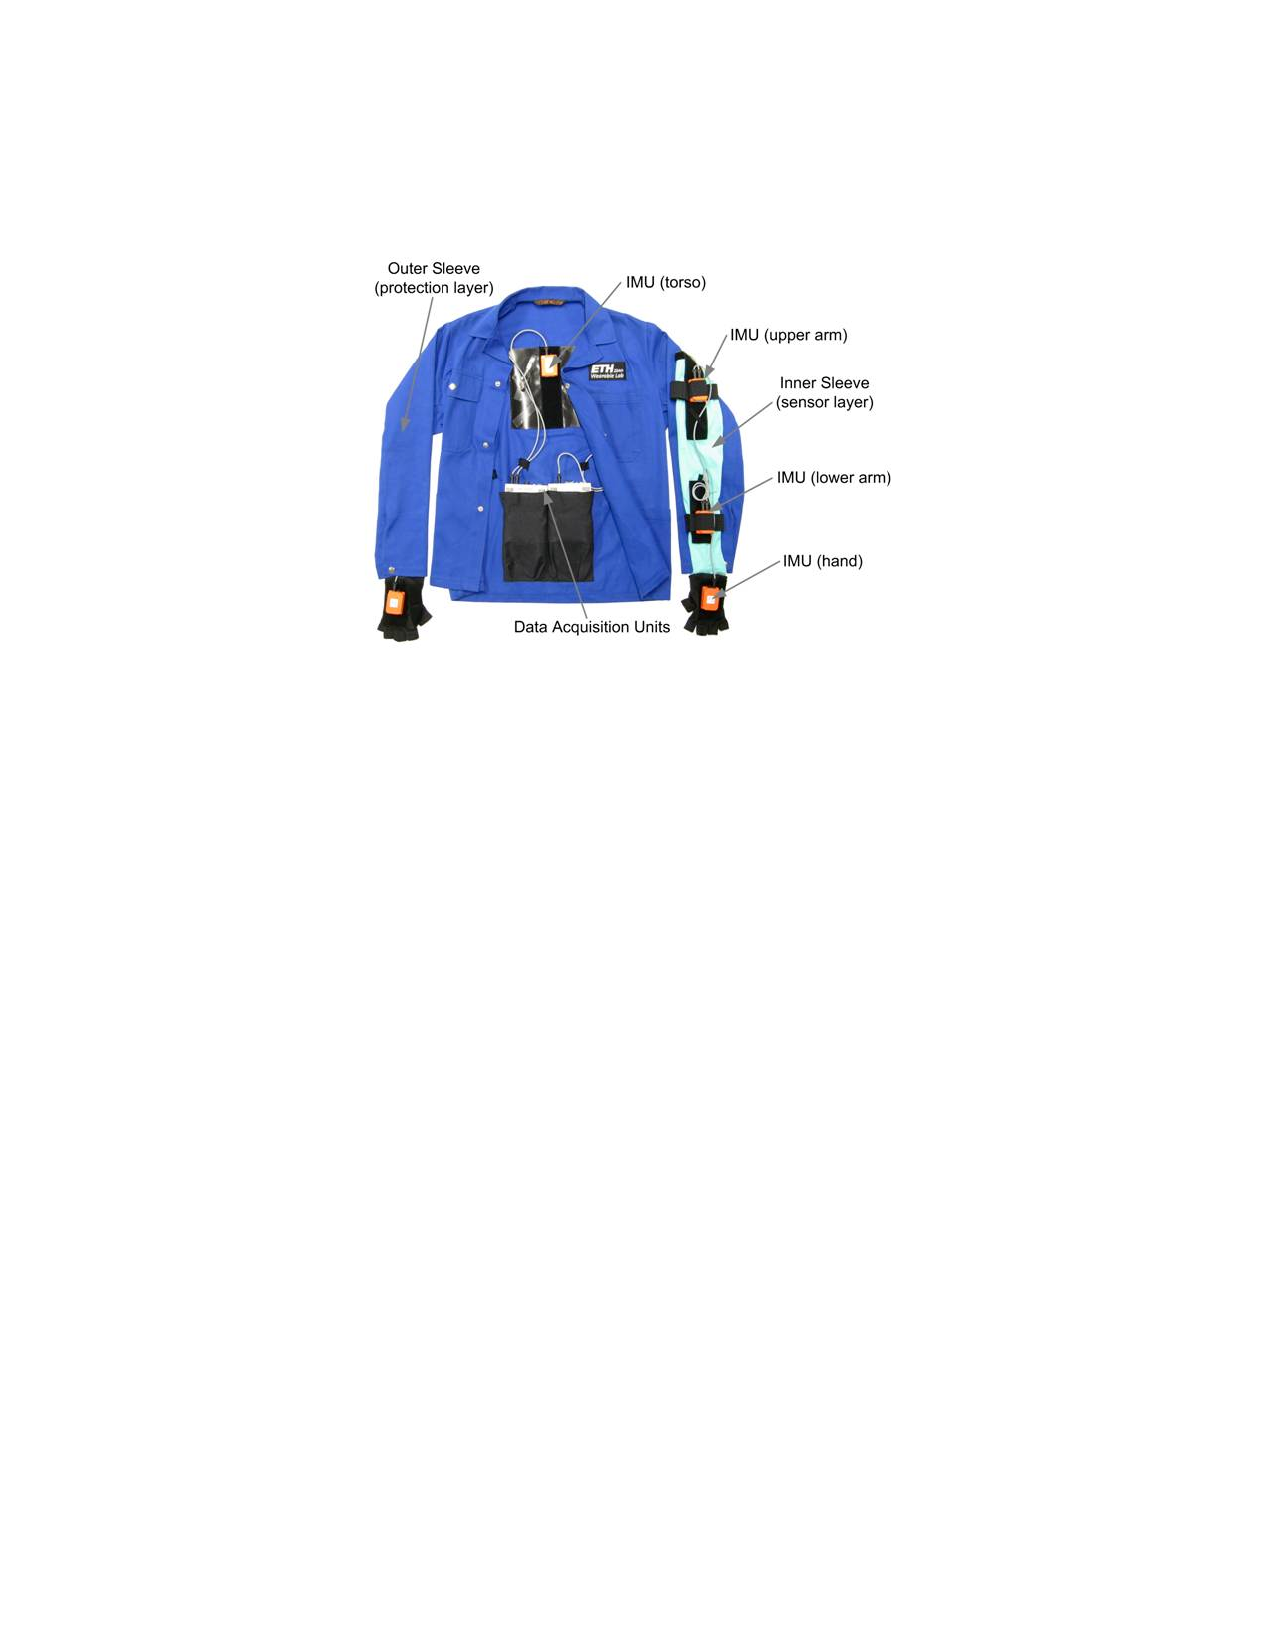
\includegraphics[width=0.5\textwidth]{images/jacket_wearable.pdf}
    \caption{Wearable motion jacket on which sensors are attached. Figure taken from \cite{opportunity}.}\label{fig:jacket}
\end{figure}

\begin{figure*} \centering
         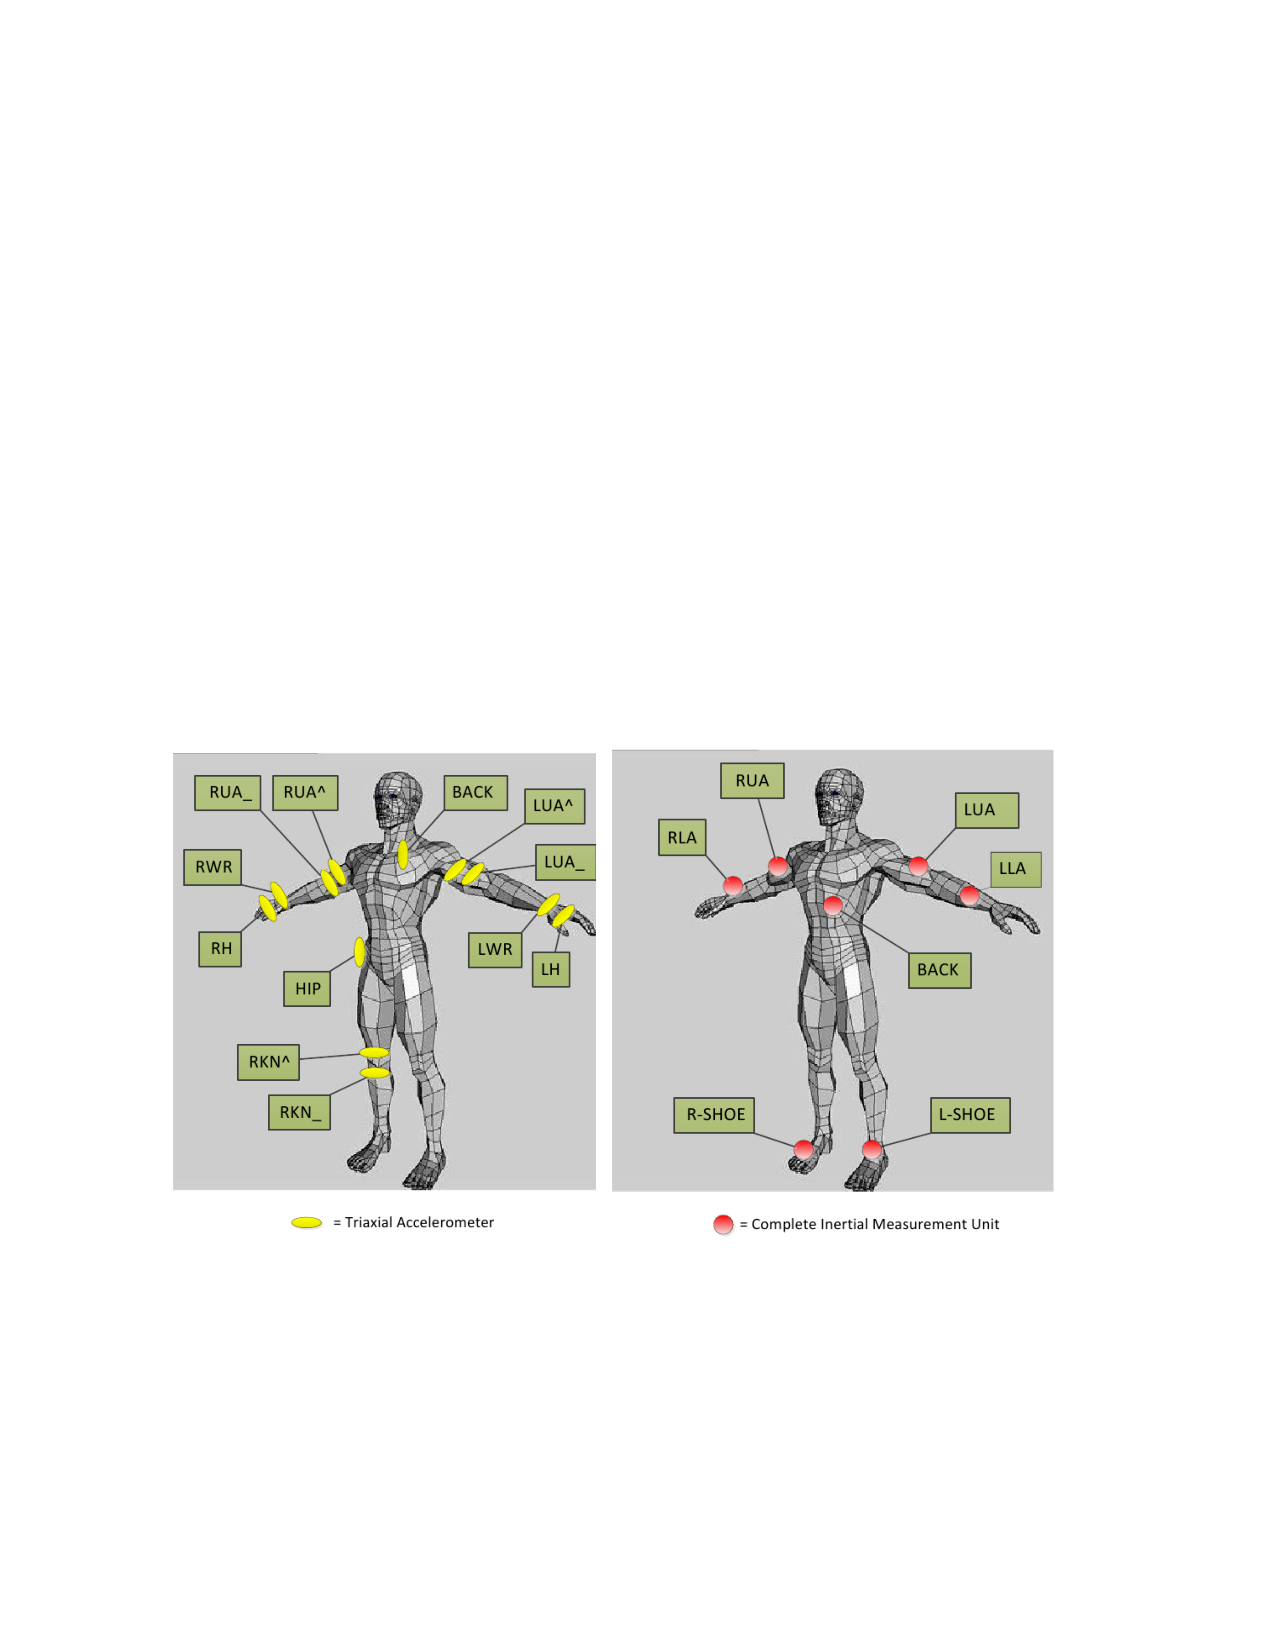
\includegraphics[width=0.8\textwidth]{images/sensors}
    \caption{Body sensor placement over the subject, for what concerns Inertial Measurement Unit on the right and Triaxial accelerometers on the left. Figure taken from \cite{opportunity}.  }\label{fig:sensors}
\end{figure*}

\subsection{Data preprocessing}
Since each of the sensor provides 3D measurements, we introduce a first approximation by taking the euclidean modulus of the three components, as follows:
\begin{equation}
M = \sqrt{x^2+y^2+z^2},
\end{equation}
for each of the considered sensors. Therefore, from now on we will always implicitly refer to the modulus instead of the single component. Moreover, let us point out that the dataset contains a non-negligible amount of missing values, nevertheless, since our analyses take into account different subsets of the entire dataset, the NaN values problem is addressed differently each time.

\section{Correlations: Principal Component Analysis (PCA)}
Let us recall that the purpose of our analysis is to provide a strategy to reduce the amount of data to share among a communication channel, with the lowest possible loss of information. To this end, we first need to show that there is indeed shared information among different signals, thus it is reasonable to approach the problem of data reduction. A possible strategy is presented by Principal Component Analysis (PCA) \cite{Jolliffe2011}, a dimensionality reduction technique which can be applied to transform data in a space of lower dimension, but also as a mathematical tool to compute how much varience of the data can be explained by means of the so-called Principal Components (PC). \par
Let us then recall a well-known quantity in the PCA scenario: the explained variance. The explained variance is a statistical measure of how much variation in a dataset can be attributed to each of the principal components generated by PCA, in the formula:
\begin{equation}
EV_i = \frac{\lambda_i}{\sum_{k=0}^{d-1}\lambda_k} ,
\end{equation}
where, $\lambda_k$ is the eigenvalue of the $k-th$ component and $d$ is the dimension of the new feature space.

\subsection{Homogeneous sensor type analysis}

For each of the sensor type, we perform a PCA \cite{sklearn_api} from a space of dimension $n$ ,without lowering the dimensionality, and we compute the explained variance. Such quantity gives indeed an estimation of how much variance of the original dataset is encoded in each component, thus, indirectly, it refers to the amount of correlation of the original features. 

\begin{figure*} \centering
         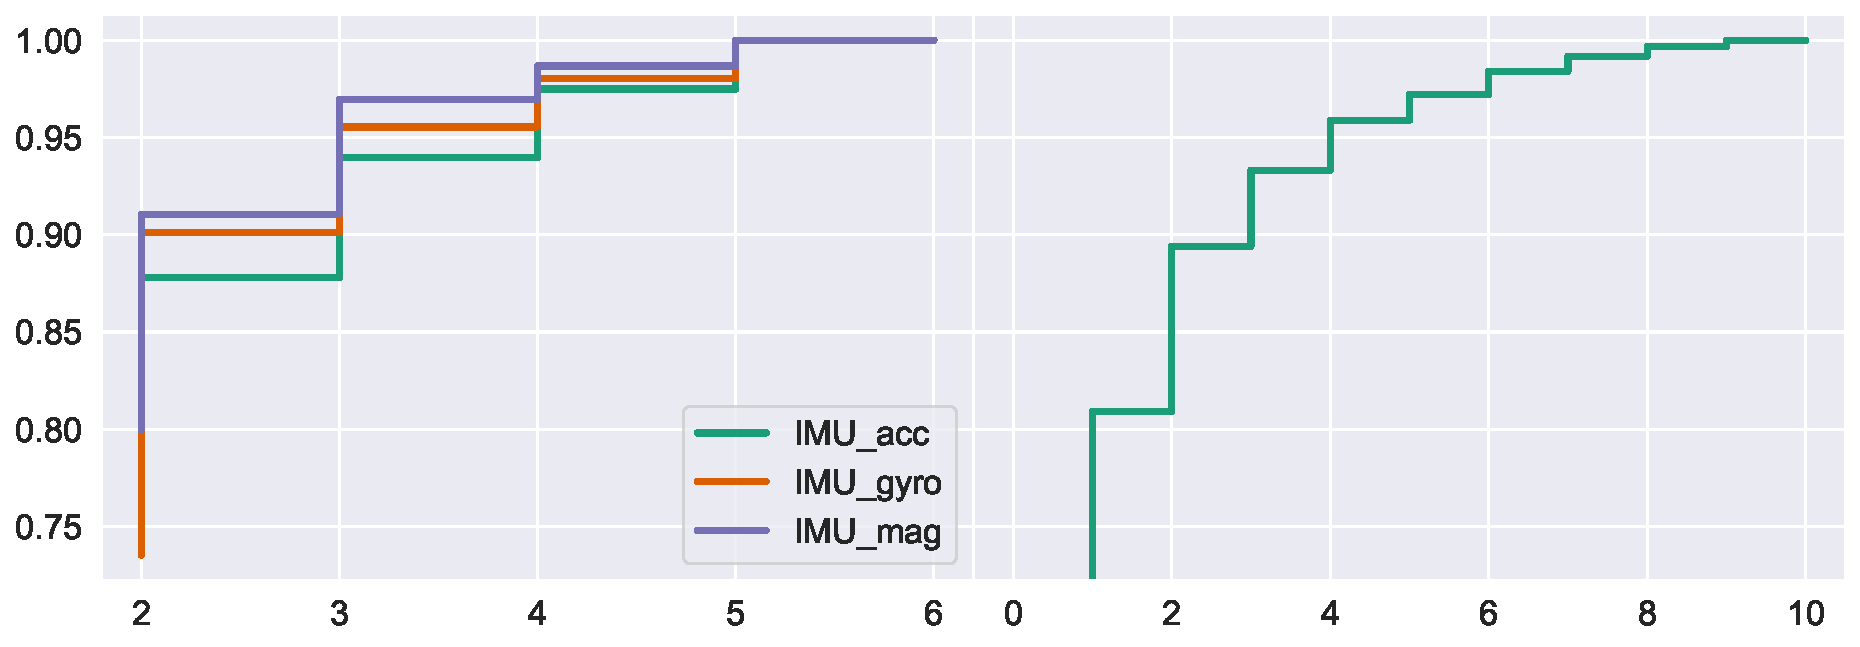
\includegraphics[width=1\textwidth]{../pca/pca_results/sub_1_run_1_ex_var.pdf}
    \caption{Cumulative explained variance of each component for subject 1, run 1. Left panel shows the explained variance referring to different IMU sensors, while right panel refers to triaxial accelerometers.  }\label{fig:pca}
\end{figure*}
 Figure \ref{fig:pca} shows an example of cumulative explained variance vs number of components considered. For what concerns the IMU signals we can highlight that, for all of them, a single component explains around 90\% of the variance, while by considering two components we are able to describe approximately 95\% of data variety. On the other hand, in order to achieve a 90\% of explained variance in the triaxial accelerometers scenario we need to consider at least two components. Therefore, since PCs are obtained by means of a linear transformation of the original features, we can assert that in the case of IMU signals a single component carries almost 90\% of the information, while for what concerns the triaxial accelerators we have to consider more components. PCA applied to different runs and subjects leads to comparable results.
 \par
From a physical point of view such observations suggest that there is high correlation among same sensor data, thus that it is possible to consider only a few sensors for each type. Clearly, more sensors are needed in the triaxial accelerometers case, since there are originally more signals to combine. On the other hand, we could use only data coming from one or two IMU sensors of each type, with a reasonable loss in terms of information.

\subsection{Heterogeneous sensor type analysis}
As a further analysis,  we consider $RUA$, $RLA$, and $BACK$ sensors for the IMU measurements and hip, back, $RUA^$, $RUA_$, $RWR$, $RKN_$ for the triaxial accelerators, and perform PCA on all these signals gathered together. Figure \ref{fig:pca_het} shows results for all the different combinations of runs and subjects.  The main outcome is that, in order to explain at least 90\% of variance in every condition, 8 components are needed in the worst case scenario.

\begin{figure} \centering
         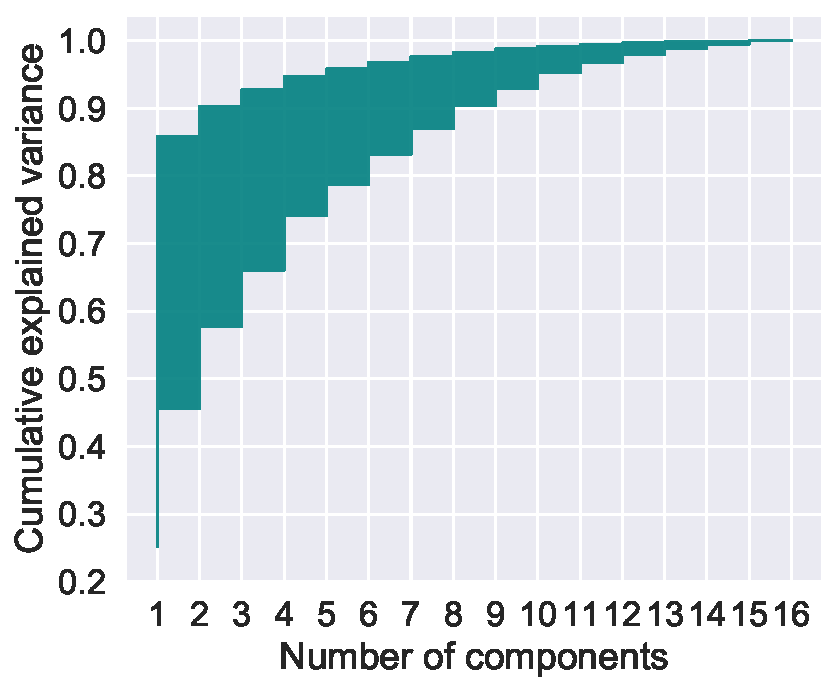
\includegraphics[width=0.5\textwidth]{../pca/pca_results/fill_global_ex_var.pdf}
    \caption{Cumulative explained variance of each component, computation performed with all the different sensor types. The filled area represents the area between the minimum and the maximum for each component, among different combination of subject and run. }\label{fig:pca_het}
\end{figure}
\vspace{0.2cm}
\par
Finally, one could argue that the explained variance refers to PCs, not to the original feature data. This is true, but since PCs are a linear combination of the physical signals, they first reflect the behaviour the latter. Moreover, one could also directly work with PCs, applying the natural dimensionality reduction induced by PCA. Nevertheless, it is relevant to highlight that PCs do not have a clear physical meaning, since these are obtained by means of a geometric transformation of the original data and live in a geometric space with a different base. 

\section{Dimensionality reduction}

\subsection{KMeans Clustering}
In the previous section we asserted that it is possible to use data coming from a lower number of sensor for each type while still preserving the variety of original signals. In this section we dive deeper into this possibility, analyzing dimensionality reduction from a different point of view: KMeans clustering \cite{kmeans} \cite{JMLR:v21:20-091}. The basic idea is that, for a given number of centers, KMeans identifies the optimal centers with reference to a given metric. These centers are referred to as centroids, and they are computed at each iteration of the KMeans algorithm, whose behaviour is based on optimizing the following loss function:
\begin{equation}
\Phi(P,S) = \sum_{x\in P} d^2(x,S),
\end{equation}
where $P$ is the set of points to be clustered, $d$ is the metric of the metric space and $S$ is the set of centers. We consider both euclidean and dynamic time wrapping distance \cite{dtw}.

\subsubsection{Same sensor type analysis}
Here we consider data referring to two locomotion activities, walking and laying, and for each millisecond we apply KMeans clustering with 1 to 4 centers. Figures \ref{fig:imuacc}, \ref{fig:imugyro} and \ref{fig:triax} shows the signals of the centers for the three types of sensors considered, i.e. accelerometers, gyroscopes and triaxial accelerometers. For what concerns IMU accelerometers, Figure \ref{fig:imuacc} shows that considering more centers does not add significant information to the single center case, since trends are reasonably overlapping. Moreover, it is possible to highlight that even considering the signals of the centers instead of the original time-series clearly allows to distinguish between the two locomotion activities. Indeed, one could just look at the amplitudes to visually discriminate if the subject is walking or laying. A similar behaviour can be identified also in Figure \ref{fig:imugyro} with reference to gyroscopes and in Figure \ref{fig:triax}
for triaxial accelerometers. Nevertheless, in this last case the addition of the second center seems to add information to the single center case. Such an observation is coherent with what we observed in the previous section when applying PCA: triaxial sensors cannot be reduced to a single signal, thus we need to consider more than one time-series to preserve the information content. Similar results can be obtained for other subjects and runs.
\par
To summarize, two main results can be highlighted: first, KMeans clustering allows us to reduce the number of signals for each sensor type, and the time-series of the centroids still allows us to distinguish the locomotion activities performed by the subject. Indeed, it is worthwhile to specify that the signals of each center are not physical, in the sense that these do not come directly from measurements, but they are computed as KMeans centroids.

\begin{figure*} \centering
\begin{subfigure}{\textwidth}\centering
         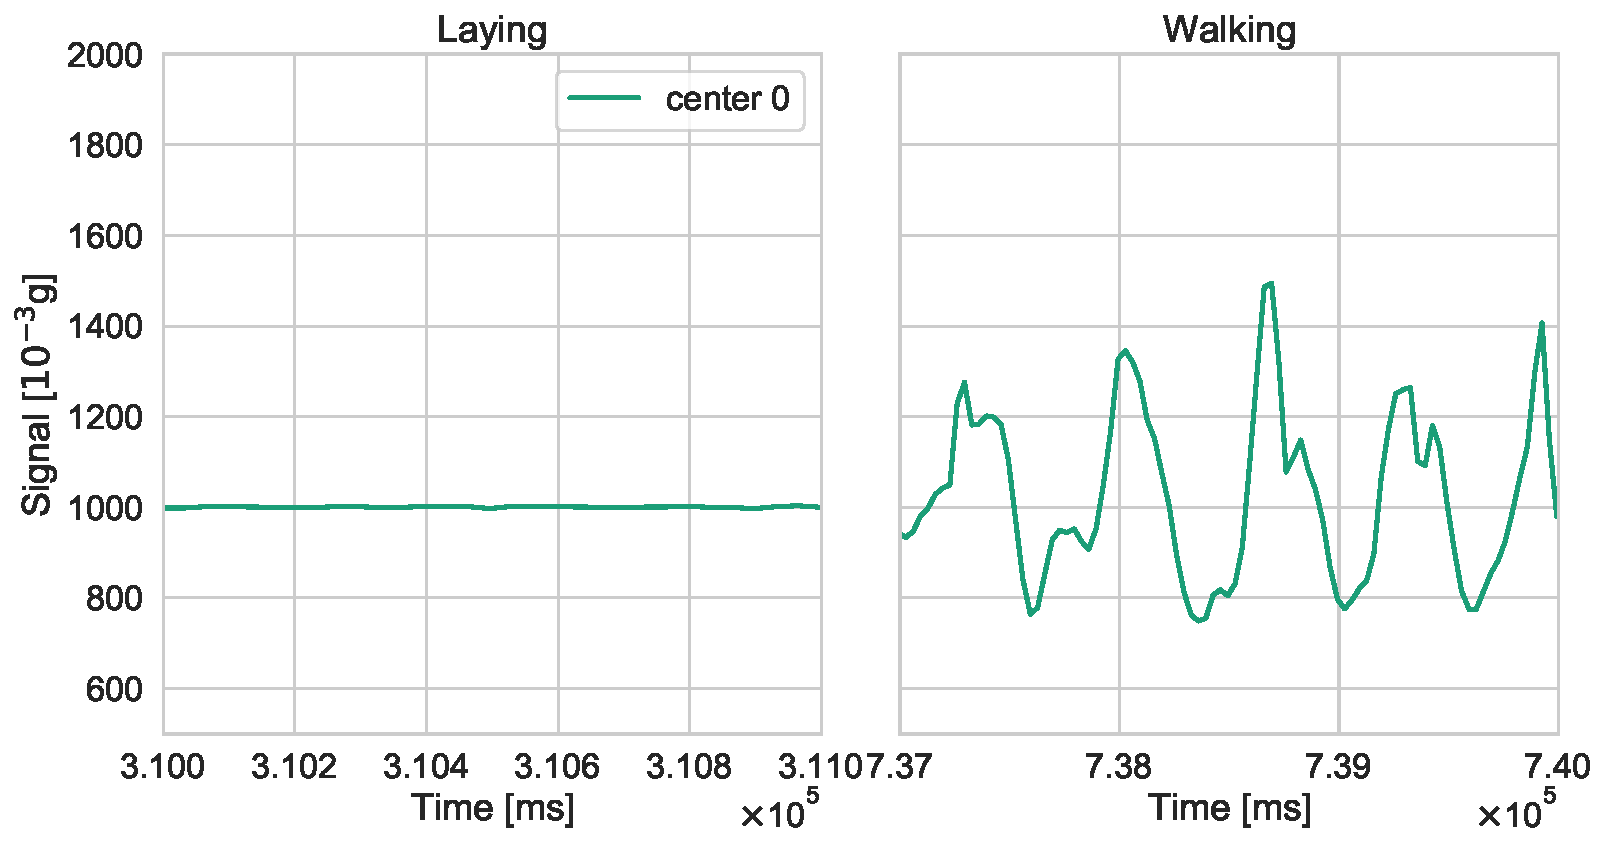
\includegraphics[width=0.8\textwidth]{../clustering/clustering_results_euclidean/subject_1/run_1/IMU_acc1_centers.pdf}
         \caption{Signal obtained with KMeans fixing 1 center.}\label{fig:imuacc1}
     \end{subfigure}
     
\begin{subfigure}{\textwidth}\centering
         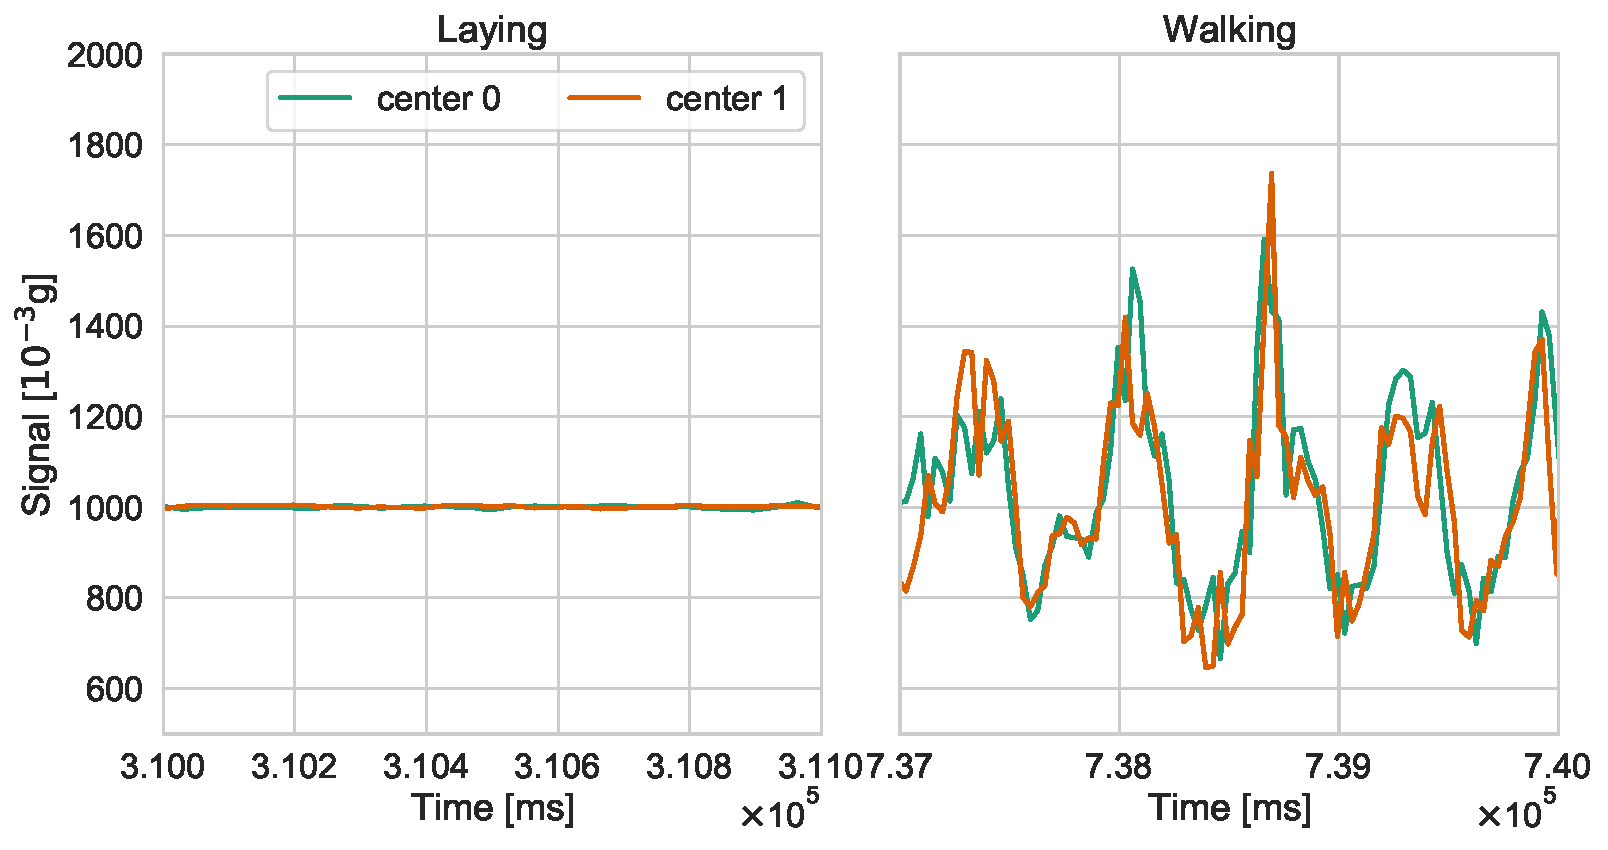
\includegraphics[width=0.8\textwidth]{../clustering/clustering_results_euclidean/subject_1/run_1/IMU_acc2_centers.pdf}
         \caption{Signal obtained with KMeans fixing 2 centers.}\label{fig:imuacc2}
     \end{subfigure}
     
\begin{subfigure}{\textwidth}\centering
         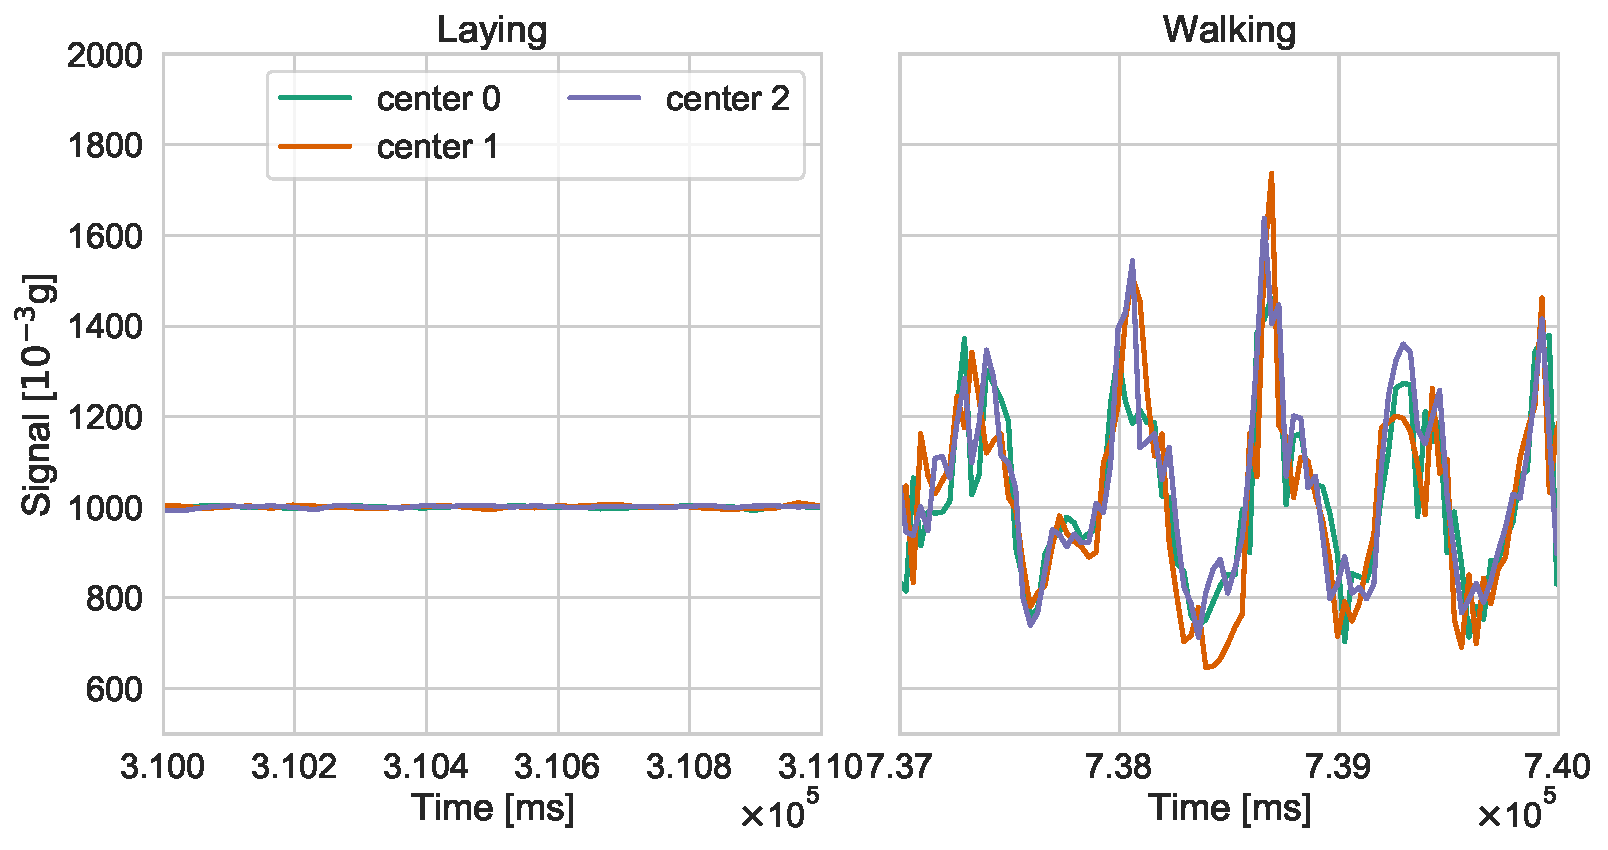
\includegraphics[width=0.8\textwidth]{../clustering/clustering_results_euclidean/subject_1/run_1/IMU_acc3_centers.pdf}
         \caption{Signal obtained with KMeans fixing 3 centers.}\label{fig:imuacc3}
     \end{subfigure}
     
  \caption{Signals of the centers obtained applying KMeans on IMU accelerometers for different numbers of clusters. Plots obtained for subject 1, run 1}\label{fig:imuacc}
\end{figure*}


\begin{figure*} \centering
\begin{subfigure}{\textwidth}\centering
         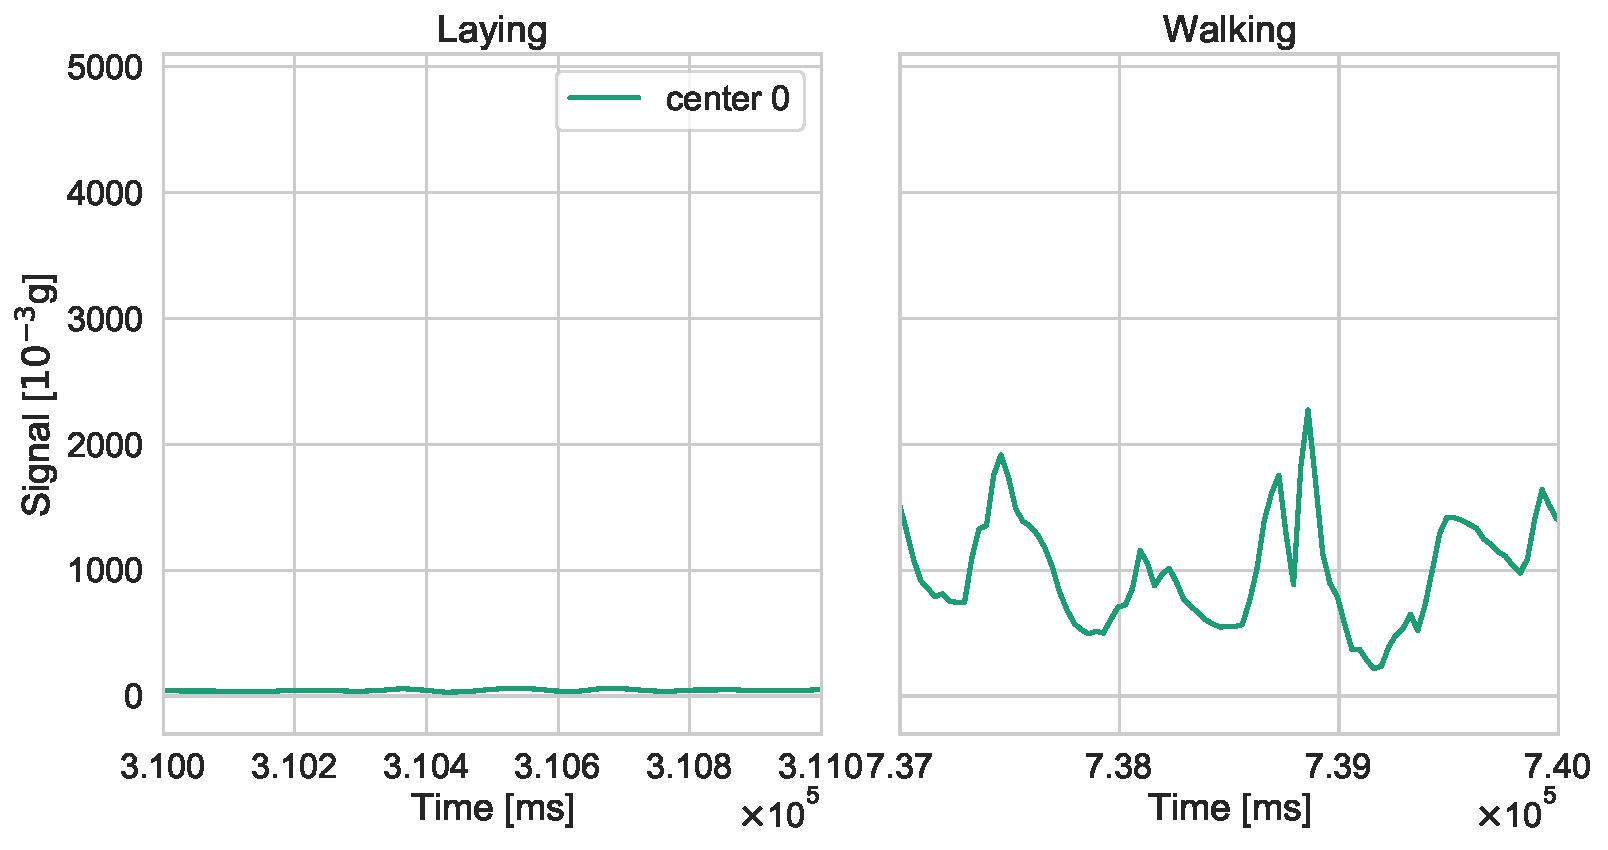
\includegraphics[width=0.8\textwidth]{../clustering/clustering_results_euclidean/subject_1/run_1/IMU_gyro1_centers.pdf}
         \caption{Signal obtained with KMeans fixing 1 center.}\label{fig:imgyro1}
     \end{subfigure}
     
\begin{subfigure}{\textwidth}\centering
         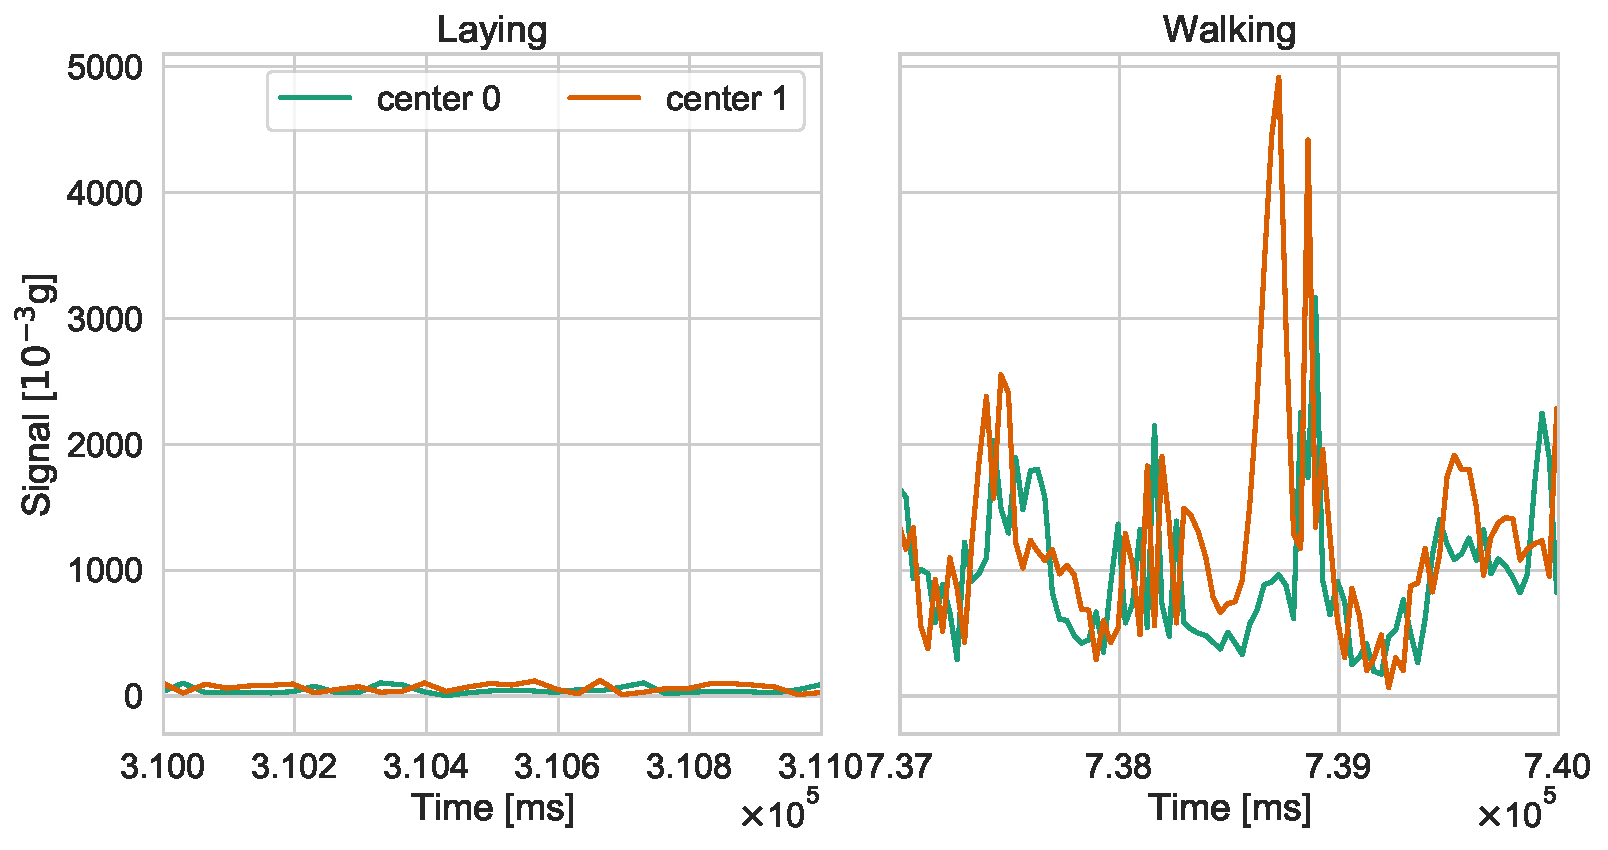
\includegraphics[width=0.8\textwidth]{../clustering/clustering_results_euclidean/subject_1/run_1/IMU_gyro2_centers.pdf}
         \caption{Signal obtained with KMeans fixing 2 centers.}\label{fig:imgyro2}
     \end{subfigure}
     
\begin{subfigure}{\textwidth}\centering
         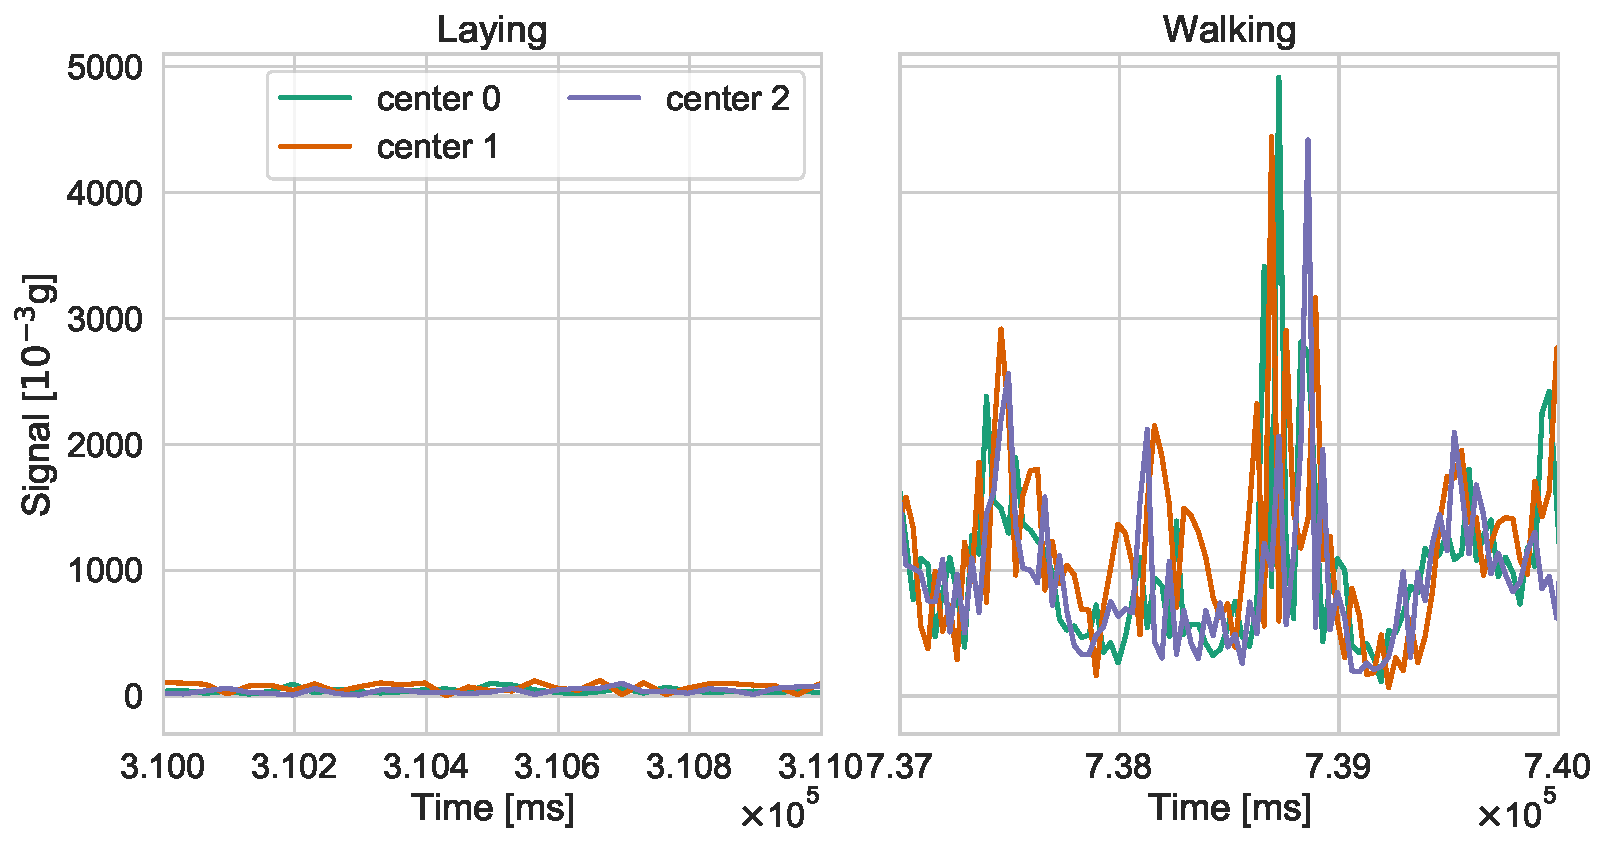
\includegraphics[width=0.8\textwidth]{../clustering/clustering_results_euclidean/subject_1/run_1/IMU_gyro3_centers.pdf}
         \caption{Signal obtained with KMeans fixing 3 centers.}\label{fig:imgyro3}
     \end{subfigure}
     
  \caption{Signals of the centers obtained applying KMeans on IMU gyroscopes for different numbers of clusters. Plots obtained for subject 1, run 1}\label{fig:imugyro}
\end{figure*}

\begin{figure*} \centering
\begin{subfigure}{\textwidth}\centering
         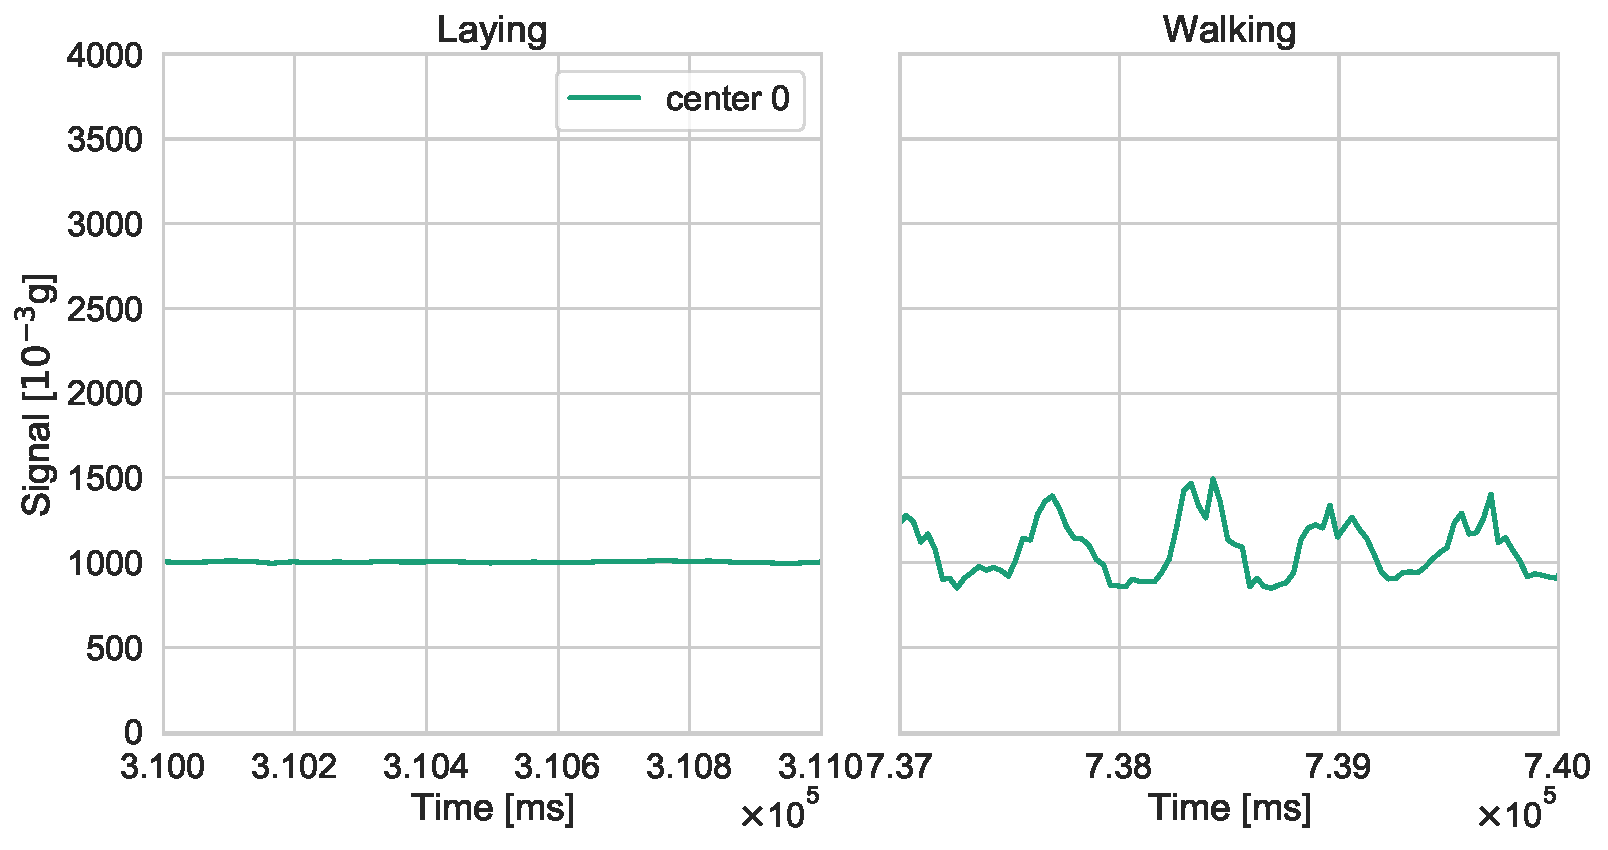
\includegraphics[width=0.8\textwidth]{../clustering/clustering_results_euclidean/subject_1/run_1/triaxial_acc_1_centers.pdf}
         \caption{Signal obtained with KMeans fixing 1 center.}\label{fig:triax1}
     \end{subfigure}
     
\begin{subfigure}{\textwidth}\centering
         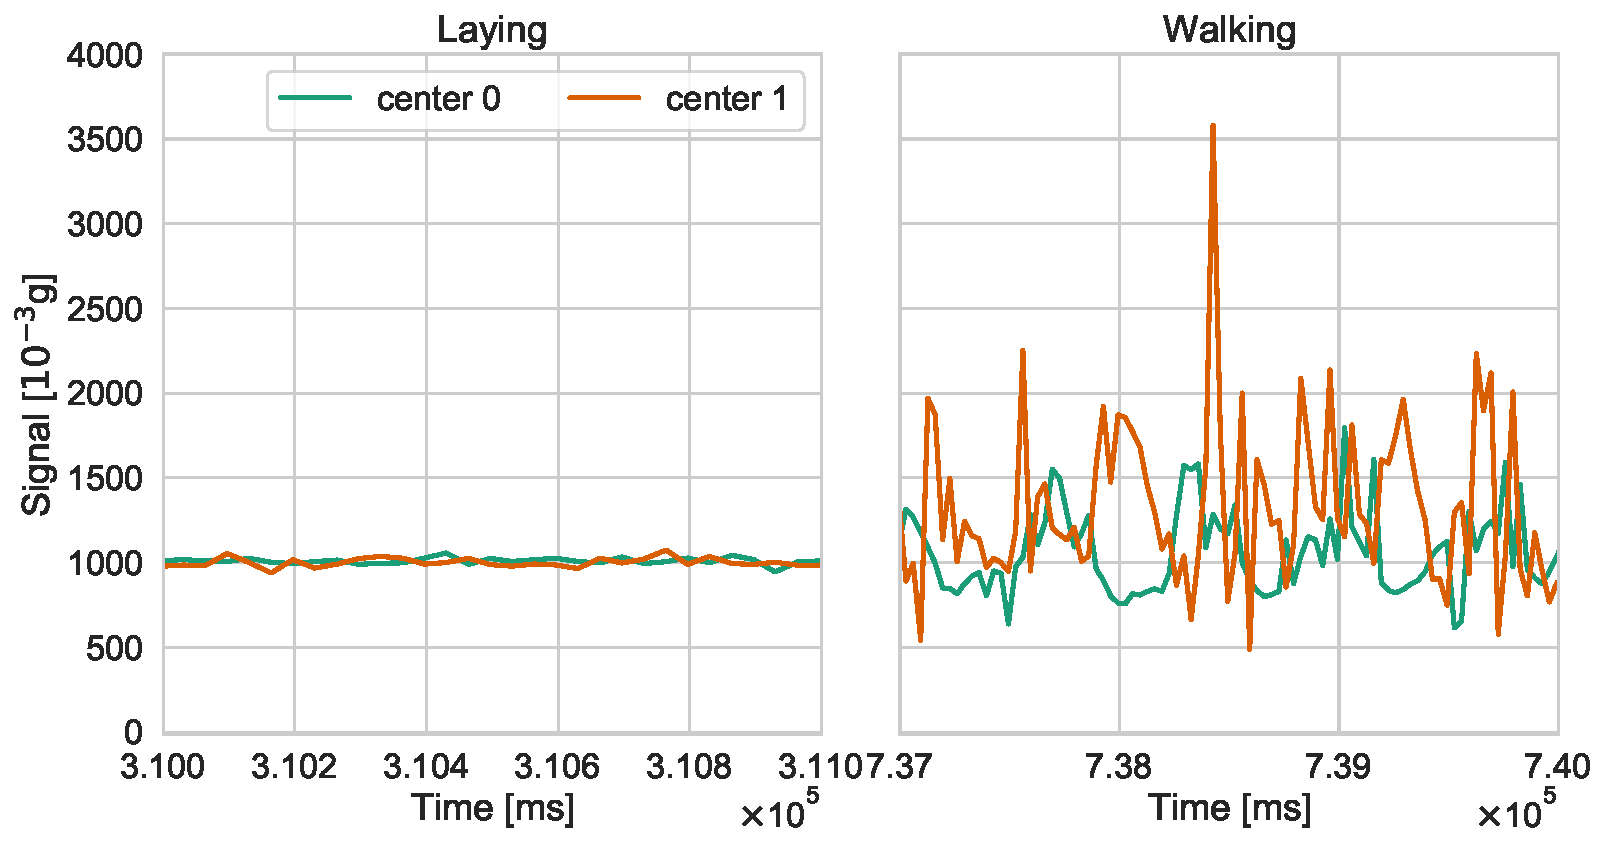
\includegraphics[width=0.8\textwidth]{../clustering/clustering_results_euclidean/subject_1/run_1/triaxial_acc_2_centers.pdf}
         \caption{Signal obtained with KMeans fixing 2 centers.}\label{fig:triax2}
     \end{subfigure}
     
\begin{subfigure}{\textwidth}\centering
         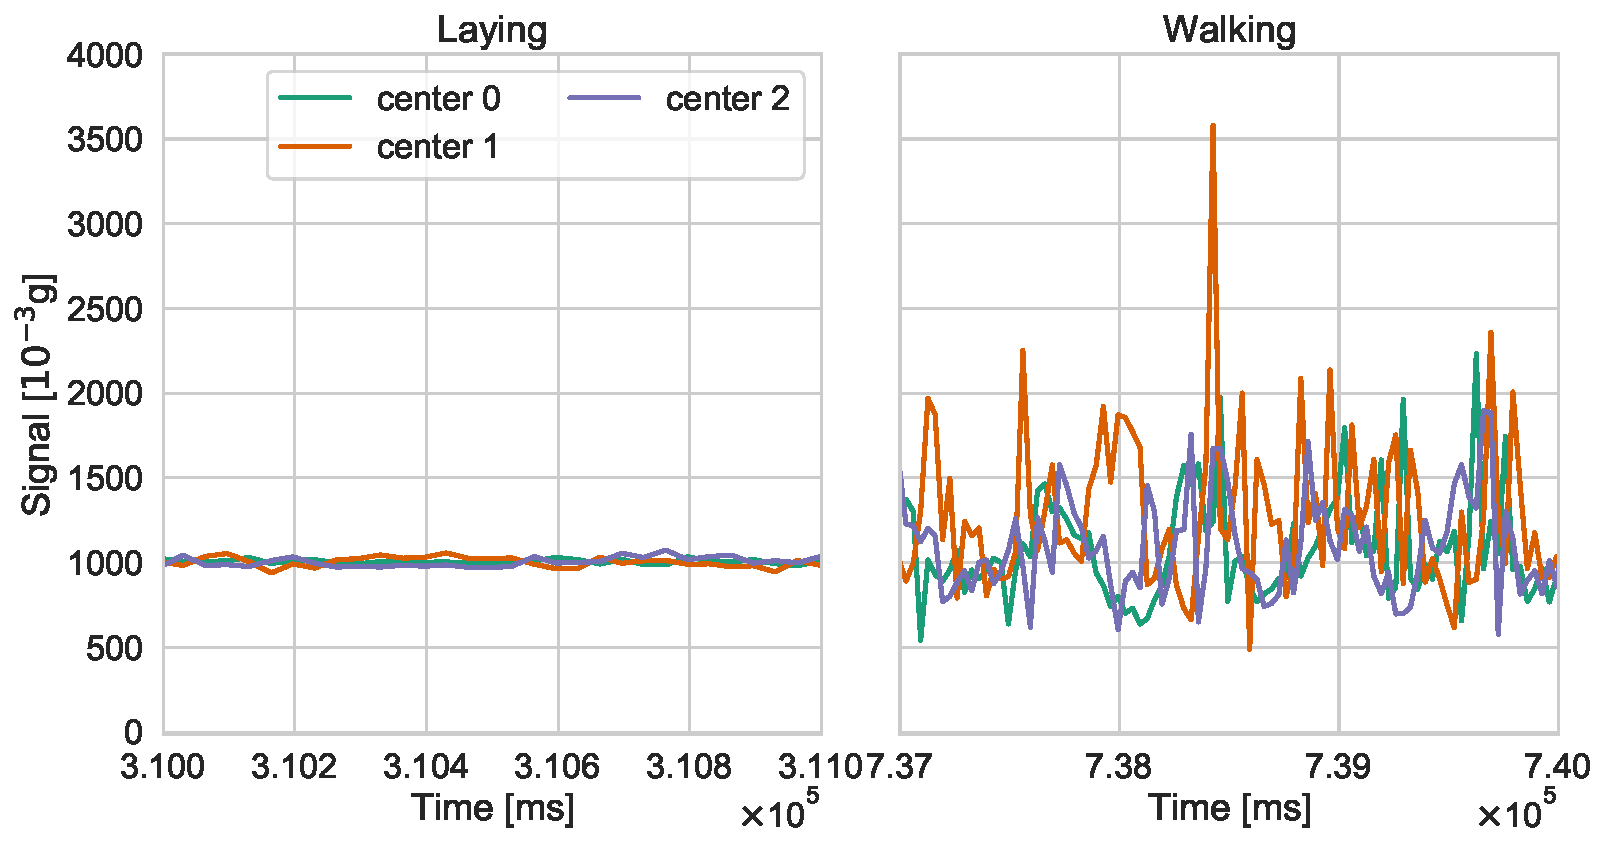
\includegraphics[width=0.8\textwidth]{../clustering/clustering_results_euclidean/subject_1/run_1/triaxial_acc_3_centers.pdf}
         \caption{Signal obtained with KMeans fixing 3 centers.}\label{fig:triax3}
     \end{subfigure}
     
  \caption{Signals of the centers obtained applying KMeans on triaxial accelerometers for different numbers of clusters. Plots obtained for subject 1, run 1}\label{fig:triax}
\end{figure*}

\subsection{Homogeneous sensor type classification}\label{sec:homo}
Clustering allows us to visually explore the effects of a dimensionality reduction. Nevertheless, we are interested in providing a quantitative estimation of the information loss. To this aim, in this section we try to give an answer to the following question: how well can we still distinguish high level activity after clustering? The approach is straightforward: we train a binary classifier, binary for sake of simplicity, on part of the original features and validate its performances on a test subset. Finally, we test the accuracy of our model on the data obtained from the signals of the centroids. \par
Two strategies are exploited: a linear classifier on the amplitude of the signals and a neural model on the entire time-series.

\subsubsection{Linear model: logistic regression}
Let us first explore an approach based on performing binary classification on the amplitudes. The main idea is to create a dataset of amplitudes labeled with the corresponding locomotion activity, walking or laying, train a logistic regression on the classification task and test it on the cluster data. 

\paragraph{Dataset extraction} For each sensor type, let us collect all the time series referring to walking, labelled as class 1, and laying subjects, labelled as class 0. We set a window of 80 ms, and for each interval we compute the amplitude of the signal as follows:
\begin{equation}\begin{split}
A_W= |{X_{max}-X_{min}}|, \quad \text{with} \\ X_{max}=\max_{x\in W }x, \quad X_{min}=\min_{x\in W }x,
\end{split}\end{equation}
where $W$ is a fixed window. \par
The same process is applied to the signals obtained from clustering. At the end we have three datasets: train data, i.e. 80\% of amplitudes extracted from original data,  test data, the other 20\%, and the clustering dataset.

\paragraph{Train and testing on original data} The model is trained and tested on the original dataset, with the results in terms of accuracy are shown in Tab. \ref{tab:regressortrain}, while confusion matrices are shown in Figure \ref{fig:cmatlogistic}. Note that, if we refer to 'walking' as positive and 'laying' as negative examples, the model shows a non negligible false positive rate. This is probably due to the fact that the amplitude is still large when there is a transition from a certain locomotion activity to laying down.

\begin{table*}[]\centering
\begin{tabular}{c|cc}
                       & test accuracy & train accuracy \\ \hline
IMU Accelerometer      & 0.96          & 0.96           \\
IMU Gyroscope          & 0.95          & 0.95           \\
triaxial Accelerometer & 0.93          & 0.92          
\end{tabular}\caption{Test and train accuracy of a linear regressor for each sensor type. }\label{tab:regressortrain}
\end{table*}

\begin{figure*} \centering
         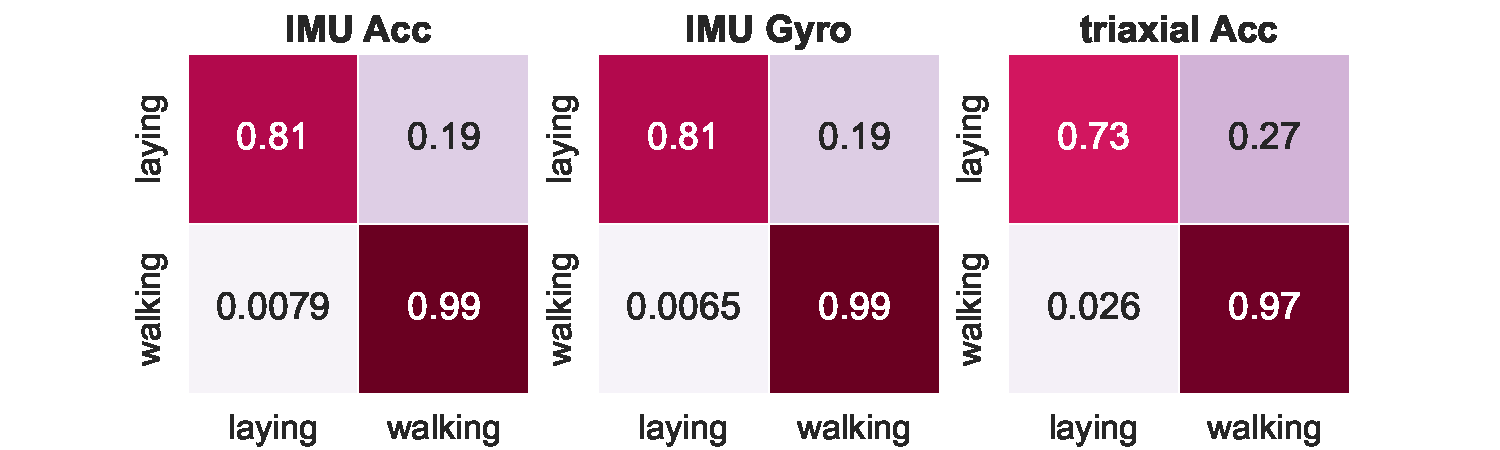
\includegraphics[width=0.65\textwidth]{../clustering/clustering_results_euclidean/confusion_matrix_test.pdf}
    \caption{Confusion matrices on test set for each sensor type logistic classifier.  }\label{fig:cmatlogistic}
\end{figure*}


\paragraph{Test on centroids amplitudes} Finally, in order to quantify how good a classification could be after applying KMeans clustering, we compute the accuracy on the centroids dataset, for each sensor and for each number of centers considered. The results are shown in Figure \ref{fig:logistic_clusters}. The main outcome is that for IMU sensors a single center allows us to distinguish the two locomotion activities with extremely high probability, while more centers are needed to reach the same accuracy in the case of triaxial accelerometers. Note that these observations are perfectly coherent with what we observed in PCA and heuristically by simply plotting the signals of the centers in Figure \ref{fig:triax}.

\begin{figure} [h]
         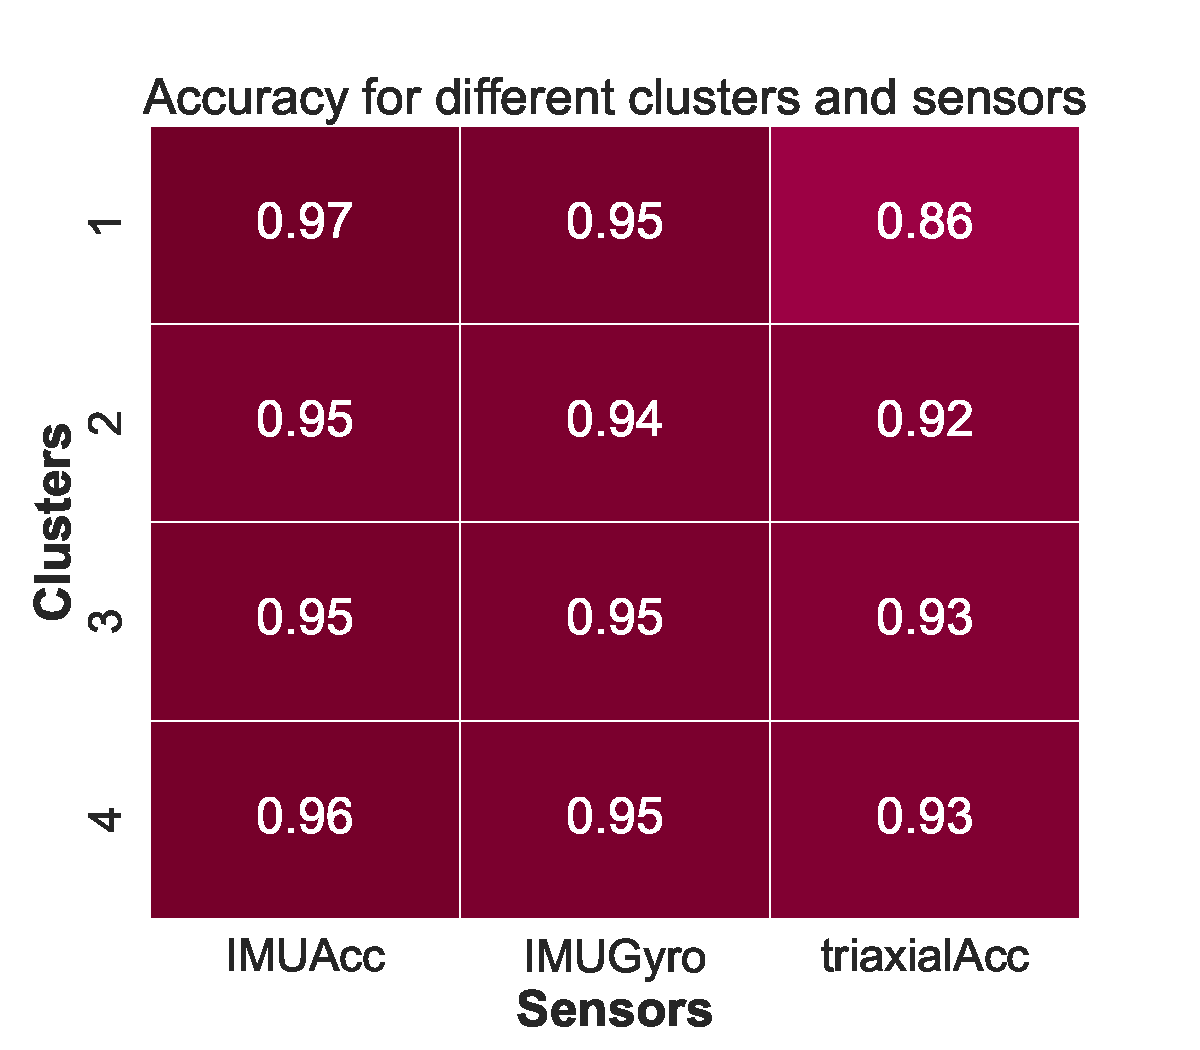
\includegraphics[width=0.55\textwidth]{../clustering/clustering_results_euclidean/accuracy_clusters.pdf}
    \caption{Accuracy of the logistic model for each sensor type and number of centers considered for clustering.  }\label{fig:logistic_clusters}
\end{figure}


\subsubsection{Neural model: InceptionTime }
Let us now explore a second approach based on binary classification of the entire time-series, and to this end, more delicate and sophisticated tools are needed. We implement a binary classifier of time-series by means of a specific Python module \cite{tsai} with InceptionTime architecture \cite{Ismail_Fawaz_2020}.
\paragraph{Dataset and training} In Figure \ref{fig:data_neural} we show the original measurements used to train the model. Training is performed with 4 epochs and a learning rate of $10^{-4}$.

\paragraph{Test on centroids time-series} Testing the neural model on the signals obtained from clustering always returns a 100\% accuracy and a diagonal confusion matrix. Thus, we may conclude that by means of neural models it is possible to distinguish with perfect precision the locomotion activity also on the clustered data. \par
Nevertheless, neural architectures are more delicate than logistic regressors, since they need to be fine tuned and usually require more computational time. As a consequence, since in an IoMT scenario we are interested in transmitting and processing data quickly and with the fewest number of assumptions possible, the logistic regression turns out to be better suited for the problem.

\begin{figure*} 
\begin{subfigure}{\textwidth}
         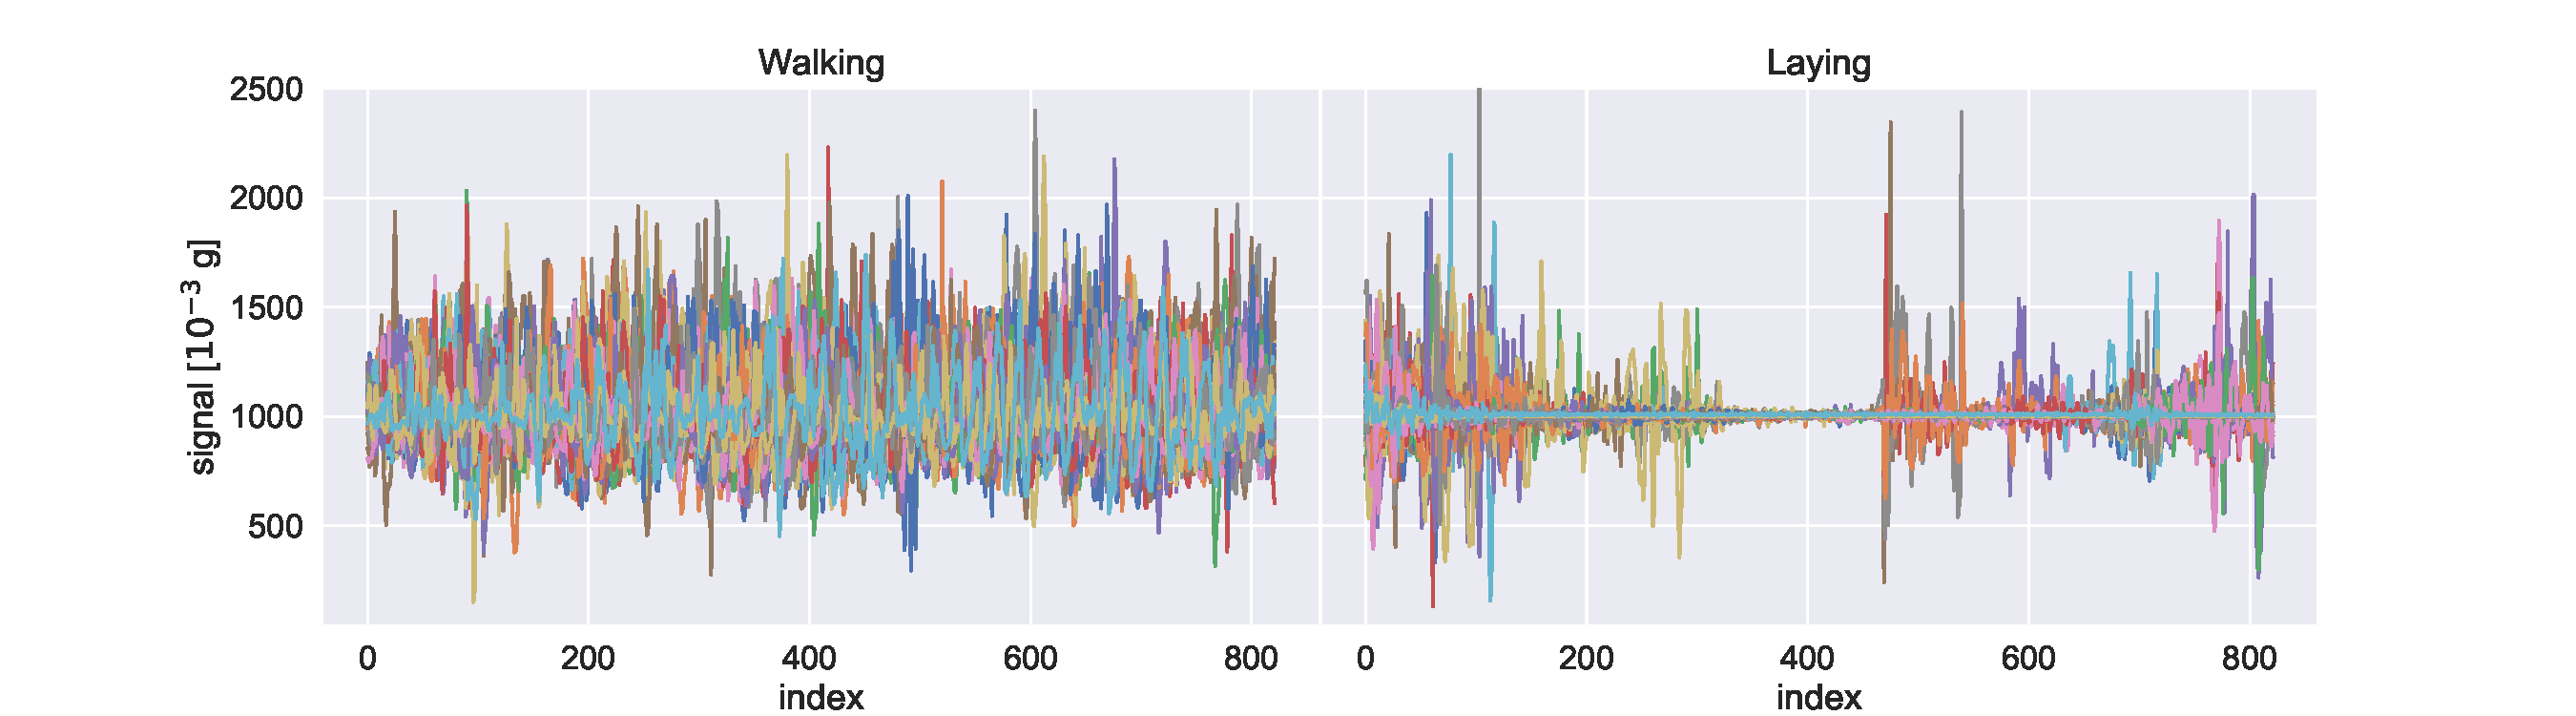
\includegraphics[width=1\textwidth]{../clustering/figures/IMU_acc_signals_walk_lie.pdf}
         \caption{Signals of IMU accelerometers }\label{fig:dataimuacc}
     \end{subfigure}
     
\begin{subfigure}{\textwidth}
         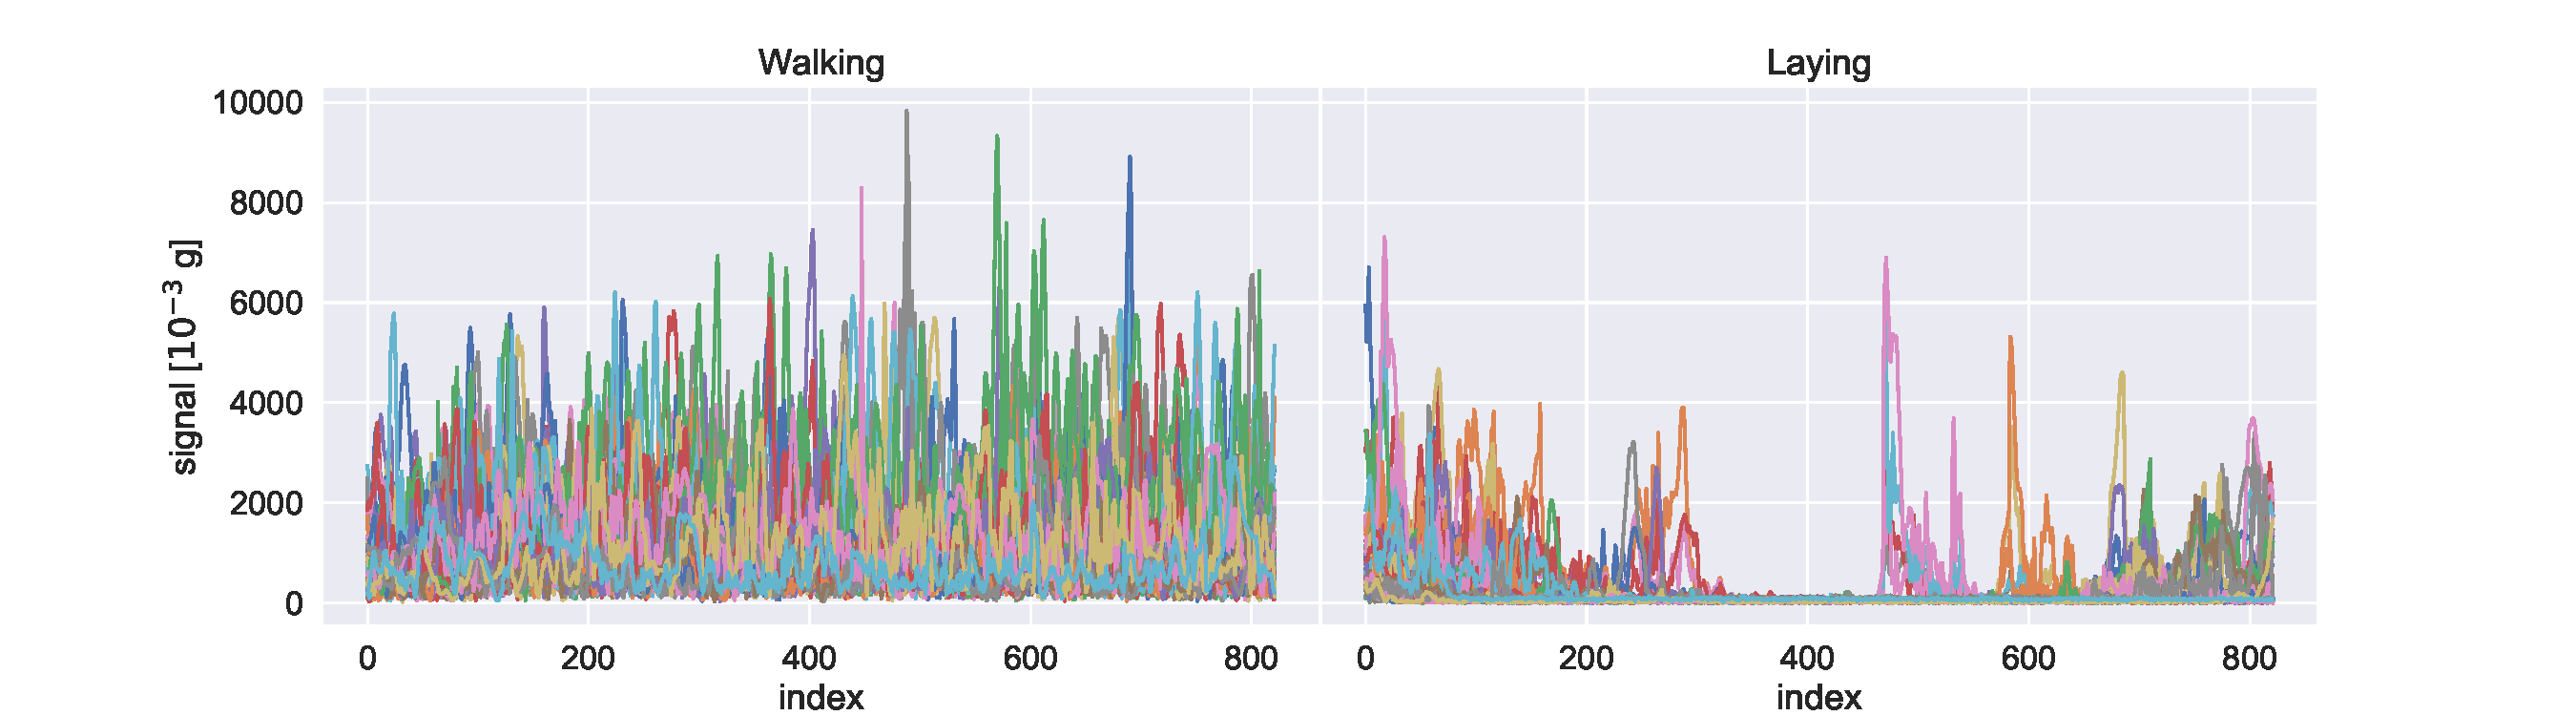
\includegraphics[width=1\textwidth]{../clustering/figures/IMU_gyro_signals_walk_lie.pdf}
         \caption{Signals of IMU gyroscopes.}\label{fig:dataimugyro}
     \end{subfigure}    
\begin{subfigure}{\textwidth}
         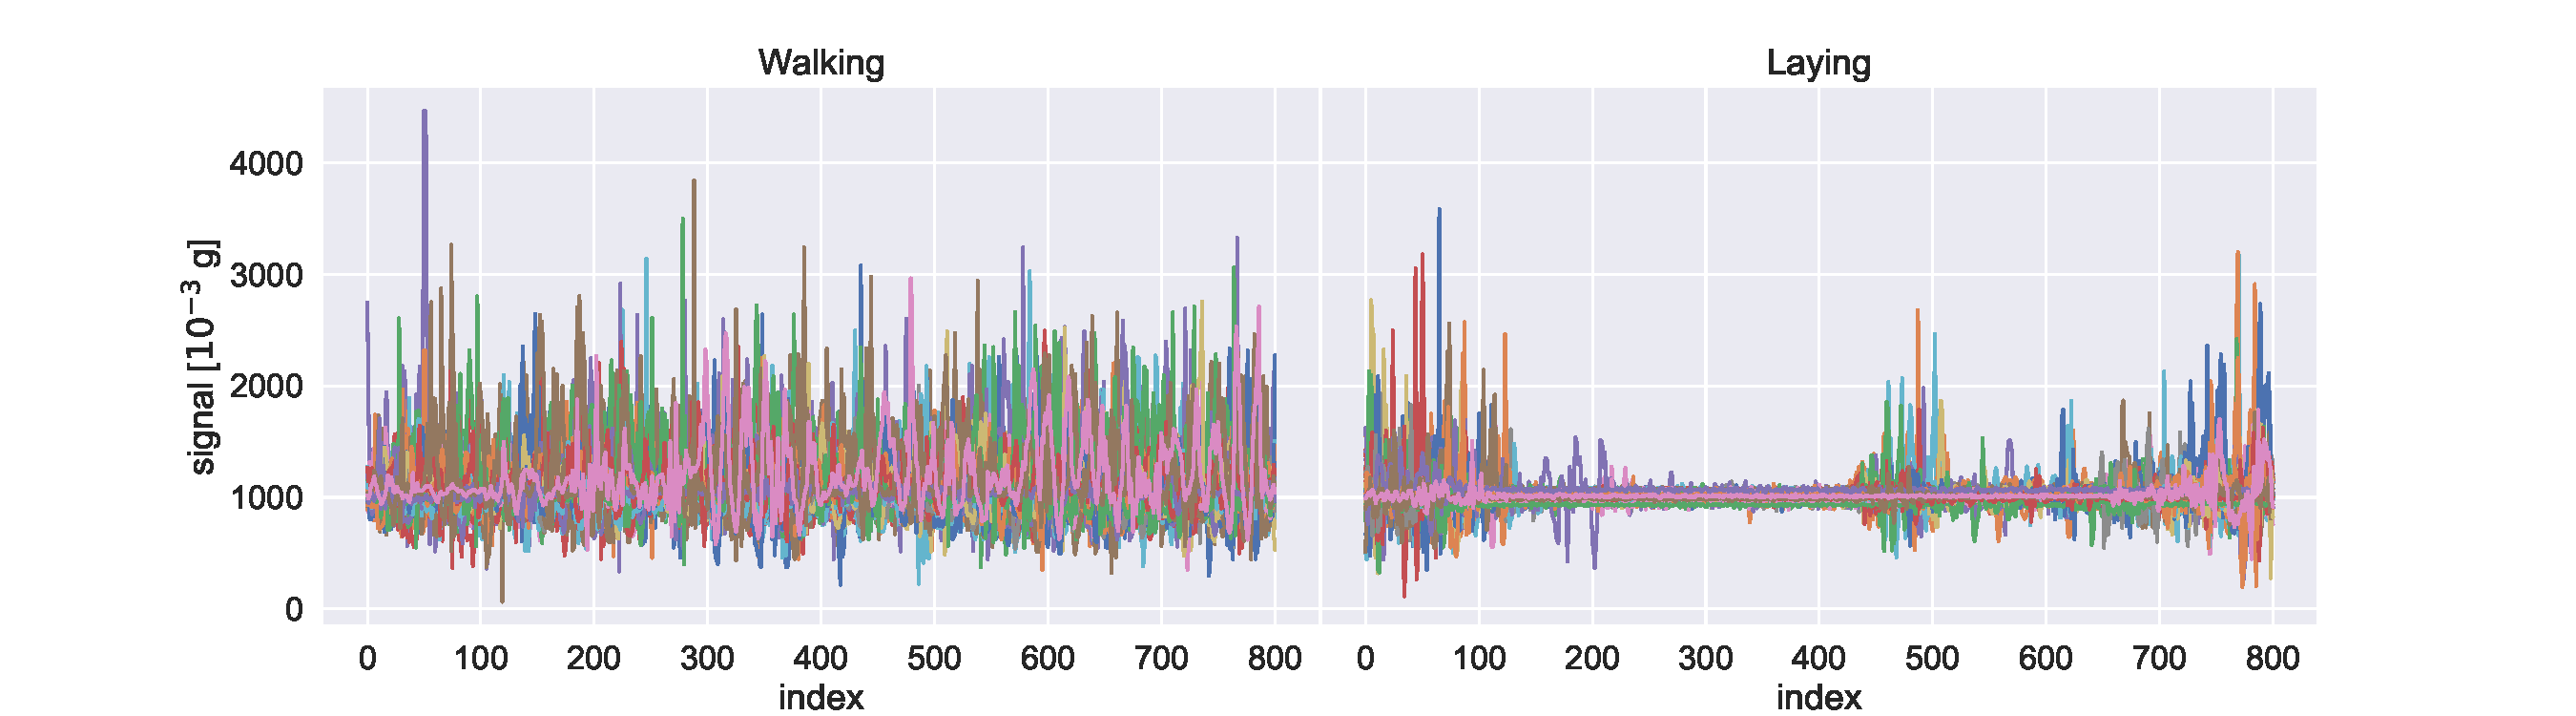
\includegraphics[width=1\textwidth, left]{../clustering/figures/triaxial_acc_signals_walk_lie.pdf}
         \caption{Signals of triaxial accelerometers}\label{fig:datatriax}
     \end{subfigure}
  
  \caption{Dataset of original signals used to train InceptionTime module for binary classification, signals are divided according to the sensor type.}\label{fig:data_neural}
\end{figure*}

\subsection{Heterogeneous sensor type classification}
Let us now consider an heterogeneous scenario, gathering data from different sensors, in particular we consider $RUA$, $RLA$, and $BACK$ sensors for the IMU measurements and hip, back, $RUA^$, $RUA_$, $RWR$, $RKN_$ for the triaxial accelerators. We apply the same process already discussed in Section \ref{sec:homo}.
Figure \ref{fig:het_linear} shows the accuracy obtained by the linear regressor on the clustering dataset for different number of clusters used in KMeans.




 \begin{figure} 

 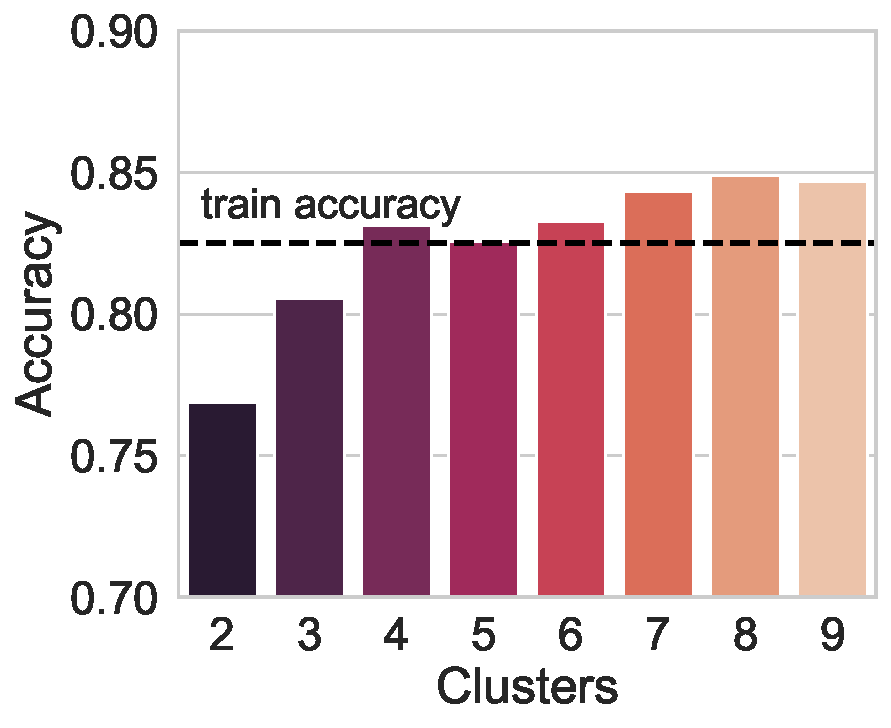
\includegraphics[width=0.5\textwidth]{../clustering/clustering_results_euclidean/heterogeneous_accuracy_amplitude_clusters.pdf}
         \caption{Linear regression accuracy in an heterogenous scenario. We consider $RUA$, $RLA$, and $BACK$ sensors for the IMU measurements and hip, back, $RUA^$, $RUA_$, $RWR$, $RKN_$ for the triaxial accelerators.}\label{fig:het_linear}
 \end{figure}
%\section{Network modelling}
%In the following sections, we will present some of the most important technologies that allow the communication through this type of networks.
%present the architecture of IoMT and
% the performance of the network
%IoT requirements and challenges
\section{Communication technologies}
After the ML analysis, we aim to project an IoMT platform to connect our sensors to the Internet. In the last few years, IoMT has faced new challenges, both in terms of network design and dimensioning. In particular, a path of research is focusing on the development of communication technologies optimized for low-power operations, i.e. long battery life, and reduced device complexity \cite{Lora_IoT}.

%In recent years, we have assisted to a kind of Revolution of IoMT with the development of compact, ultra low-power sensor devices and lightweight communication protocols that allow real-time patients monitoring with a decision support system at the hospital. They are the so-called Medical Things. 
In order to achieve such purposes, various supported connectivity solutions have been developed. Each proposed technology relies on the usage of different range, data rate, power restrictions, encryption level, coding and transmission schemes, modulation and several other aspects.
\Par
Therefore, in the following sections, we explore one of the most promising technologies in the field. In particular, we decide to focus on long-range communication technologies with low energy consumption requirement, the LPWA (Low-Power Wide Area) technologies \cite{wearable}. We perform a simulation and set realistic parameters for our problem. The main analysis focuses on studying network metrics, e.g. throughput and packet error rate (PER), for different numbers of sensors that transmit information. Eventually, we compare these values with the accuracy obtained with the ML analysis.
\\
\subsection{LPWA technologies}
The IoT communication range can cover several tens of kilometers, since a typical IoT scenario is required to work in large operation area. % as the end devices are distributed.
Therefore, wireless devices need more power supply to communicate over large distance. Due to such issue, it is critical for IoT applications to employ low-complexity and low-cost end devices, in order to perform low power operations. A possible strategy to address these problems is offered by Low-Power Wide Area Network technologies (LPWANs), which have the capability to implement architectures with the characteristics required by an IoT scenario. \cite{Lora_IoT}.
\\
\begin{figure*}
    \centering
    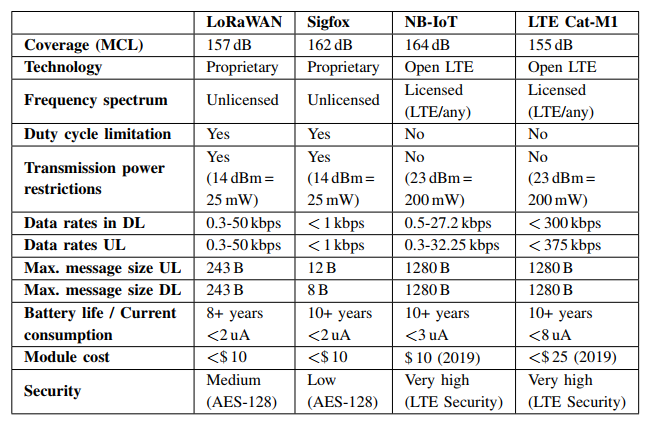
\includegraphics[scale = 0.7]{images/Characteristics.PNG}
    \caption{LPWAN technologies.}
    \label{fig:technologies}
\end{figure*}
Moreover, in recent years, several technologies have been developed to achieve sustainable coverage for large scale IoT devices, both in the licensed and in non-licensed spectrum \cite{experimental_evaluation}.
In the licensed band, we have LTE-M and narrowband IoT (NB-IoT). On the other hand, in the unlicensed bands, SigFox and LoRa are two prominent technologies, which are increasingly deployed in different IoT applications.
\par
For instance, in 2018, Global Market Insight published a market research that showed the recent increasing of the LPWAN market. In particular, at the state of art LoRaWAN has the biggest portion of the market share, approximately 50 \%. Thus we decide to focus on the LoRa technology for our analysis. Nevertheless, it is worth to highlight that NB-IoT is expected to get to the 30 \% of the market share by 2025 \cite{market}. 

\subsubsection{LoRaWAN}
LoRaWAN is a Low Power and Wide Area networking protocol based on LoRa technology, in order to connect battery operated device to the internet \cite{Lora_IoT}.  

It is designed to wirelessly connect battery operated ‘things’ to the internet in regional, national or global networks.
 The network architecture of LoRaWAN is usually a star-of-stars topology in which gateways deliver messages from end-devices to central network server and vice versa \cite{Lora_IoT}. Figure \ref{fig:Lora_architecture} shows the LoRaWAN architecture with End-Devices, Gateways, Network Server and Application Server.
 
 %The connection between gateways and the network server uses Internet Protocol standard connections. The gateways serve as transparent bridges as well as transforming the Radio Frequency packets to the IP packets. The wireless communication take the benefit of the LoRa phy-layer characteristic that enabling a single-hop link between gateways and the end-device.
%the EDs connected to the network server via gateways (GWs) that relay data between EDs and network server (NS).
\\
\begin{figure*}
    \centering
    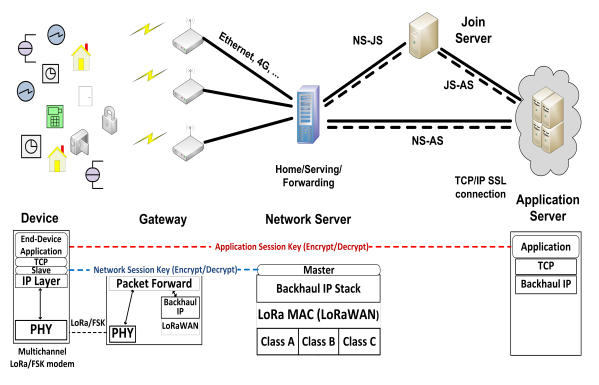
\includegraphics[scale = 0.9]{images/LoRa_arch_new.PNG}
    \caption{LoRaWAN Netowrk Architecture.}
    \label{fig:Lora_architecture}
\end{figure*}
To provide long-range communication, LoRaWAN uses LoRa modulation which is based on Chirp Spread Spectrum (CSS). Moreover, it provides a data rate varying between 300 bps and 50 kbps. The maximum payload is 243 bytes and the number of messages transmitted both in the Uplink and in the Downlink per day is unlimited. The battery life of end devices can go beyond 10 years \cite{comparative_study}.%LoRaWAN network architecture is generally a star-to-stars topology illustrated in Figure \ref{}, in which GWs seamlessly relay data between EDs and NS.
\\
Now that we have introduced the theoretical scenario, in the following section we are going to simulate a simple LoRaWAN with NS-3, on the basis of the parameters of the OPPORTUNITY IoMT scenario \cite{experimental_evaluation}.


\section{LoRa NS-3 simulation}
Let us consider the scenario offered in the OPPORTUNITY dataset, in which data is generated every 33 ms. If each sample is quantized at 32 bits, every sensor would approximately produce samples at a rate of 960 bps. This is just a possible approach, eventually one could explore other possibilities. In \cite{typical_values}, we found that a typical IoMT data rate has an order of magnitude of a few hundreds bps, as we can see in Figure \ref{fig:typical_vaulues}. Therefore, we decided to assume that our sensor sends data at a rate with an order of magnitude of thousands of bits per second. This is compatible with the choice of the LoRaWAN technology, which makes available a data rate that goes from 300 bps to 50 kbps.


%Since this is just an hypothesis we make, we performed research in order to understand which data rate could be suitable, or at least typical in the context of IoMT. %We do not have any information about the data rate at which data were sent by sensors, 


\begin{figure*} \centering
         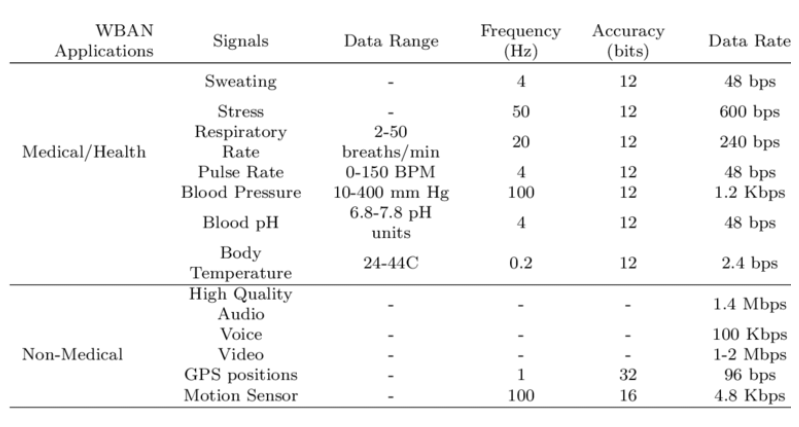
\includegraphics[width=0.9\textwidth]{images/WBAN_values.PNG}
        \caption{Typical data rate in wearable wireless sensor networks in IoMT.}
    \label{fig:typical_vaulues}
\end{figure*}



%Since we know that the sampling frequency of each sensor of the OPPORTUNITY dataset is 33 ms

\subsection{Implementation}

To simulate the network with sensors, we use the LoRa simulator projectLoRaWAN \cite{LoRa_repository}, based on the initial version of a code developed by the Signet Lab at University of Padova \cite{Signet}. The parameters are shown in Table \ref{tab:param}.



\begin{table}\centering
\begin{tabular}{llll}
\textbf{Simulation parameters} & Values\\ \hline
\textbf{Data Rate} & 1000 bps\\
\textbf{Gateway} & 1\\
\textbf{End devices} & from 4 to 86\\
\textbf{Radius} & 7000 m \\
\textbf{Simulation time} & 15 s  
\end{tabular}
\caption{Simulation parameter. }\label{tab:param}  
\end{table}

\par 
Let us consider a smart city scenario with several buildings, in which we introduce a channel model with two non-idealities: path loss and shadowing. In such scenario the End Devices, i.e. sensors, are created. Since we assume that these are worn by a person, sensors are placed in the same starting position at a height of 1.2 m and connected to the channel. Moreover, the gateway node is set in the position (0 m, 0 m, 15 m) and connected to the channel. Finally, the application is installed on the End Devices in order to generate a packet of size 23 bytes every second.



%created with the GridBuildingAllocator.

%Then we created the , respectively with LogDistancePropagationLossModel() and CorrelatedShadowingPropagationLossModel(). Then we created all the helpers related to Lora at different layers, such as LoraPhyHelper, LorawanMacHelper, LoraHelper, NetworkServerHelper and the ForwarderHelper.




%After setting the spreading factor that controls the chirp rate, and thus controls the speed of data transmission, we completed the configuration.


\subsection{Simulation and results}

The network is simulated 10 times, each time with different seeds, for each number of devices. After the run, for every fixed number of sensors, we take the average of the metric among all 10 simulations. In Figure \ref{fig:simulation}, we can see the outcomes of the simulation, in terms of packet error rate and the throughput.


\begin{figure*}\centering
\begin{subfigure}{0.50\textwidth}
    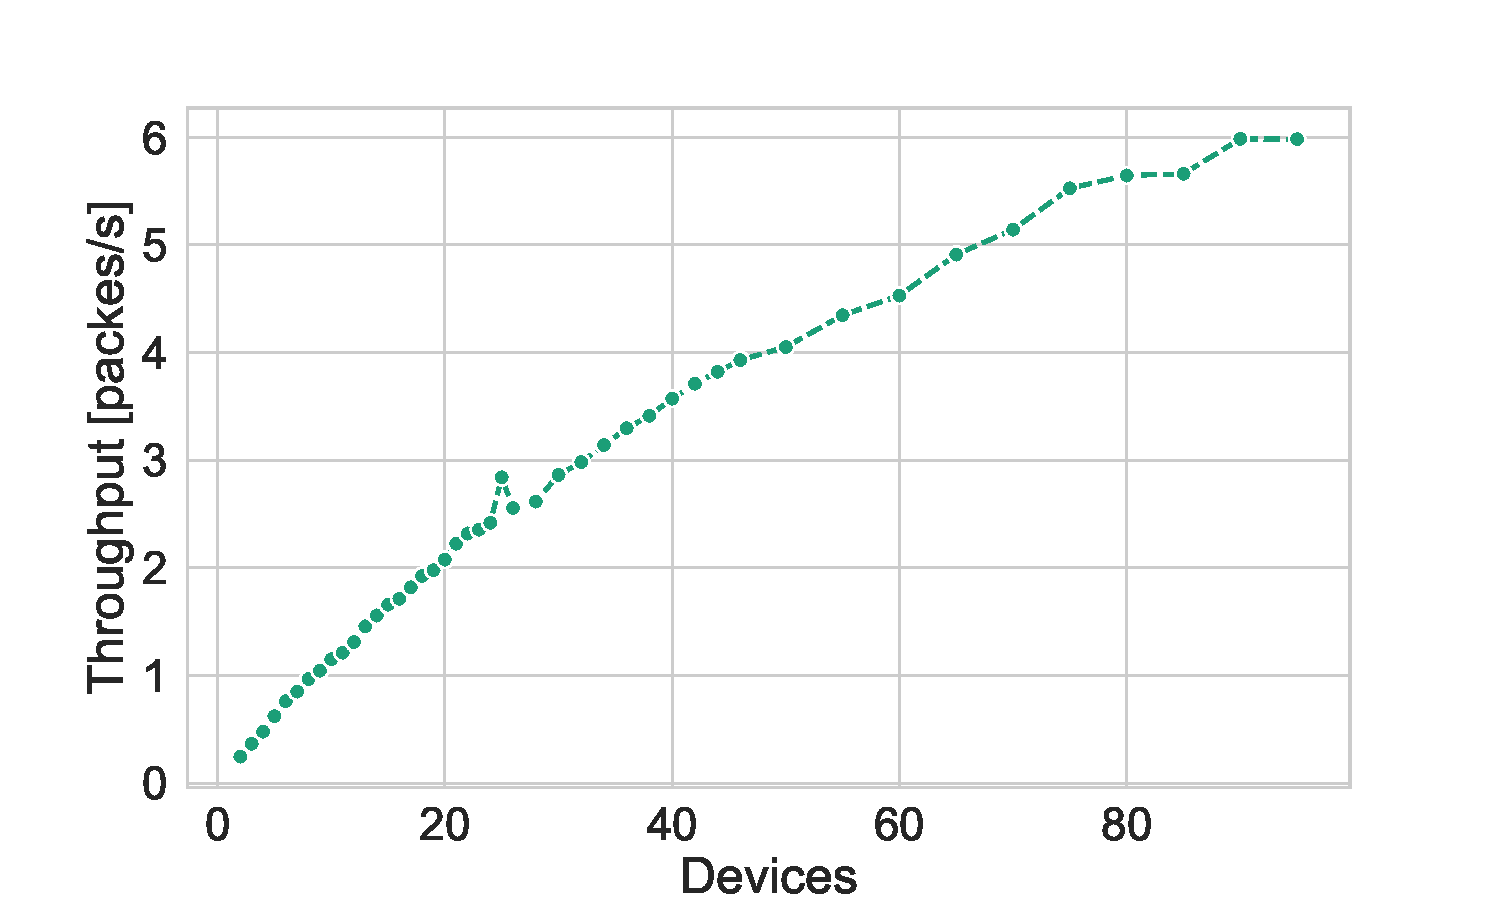
\includegraphics[scale=0.40]{images/lorawan_throughput.pdf}
    \caption{Throughput of LoRaWAN simulation.}
    \label{fig:throughput}
\end{subfigure}

\begin{subfigure}{0.50\textwidth}
    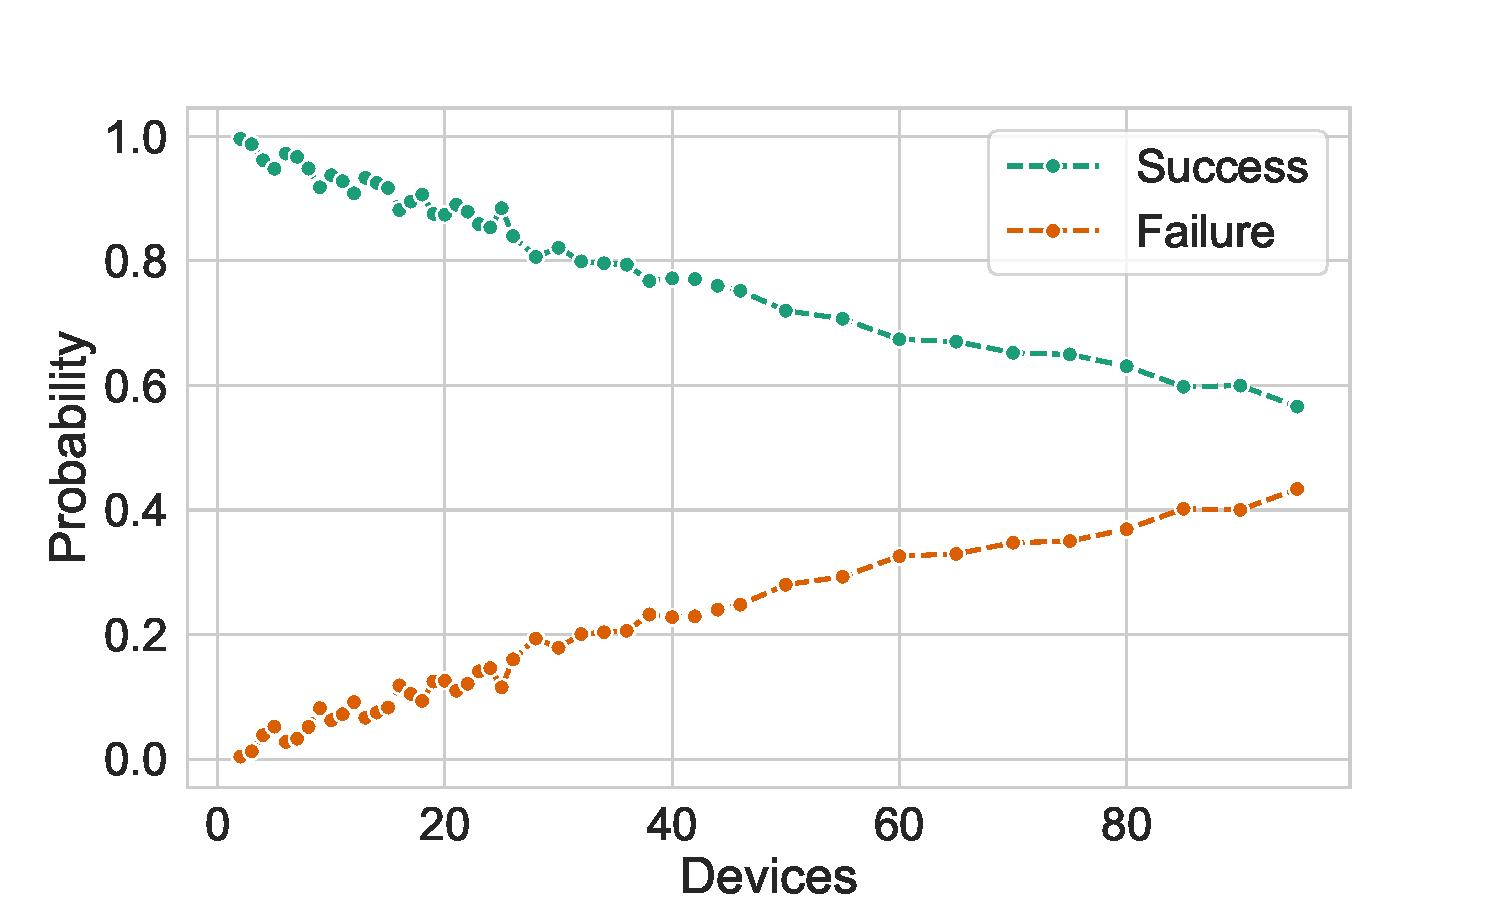
\includegraphics[scale=0.40]{images/lorawan_prob.pdf}
    \caption{Probability of success and failure in LoRaWAN simulation.}
    \label{fig:PER}
\end{subfigure} 
\caption{LoRaWAN simulation outcomes: throughput and packet error rate (PER).}
\label{fig:simulation}
\end{figure*}

As expected, Figure \ref{fig:throughput} shows that the throughput increases with the number of end devices connected. Nevertheless, we need to highlight that the considered number of sensors can still be managed by the network without overloading its capacity. For what concerns the Packet Error Rate, we can notice that it grows as soon as the number of end devices increases, see Figure \ref{fig:PER}.

At this point it is worthwhile to go back for a second to the original concern of this work: how do we find the proper trade-off between information loss and the capacity of a network?

Even though we consider a simple scenario, we can still perceive several benefits due to the reduction of the number of signals that are shared among the channel. In particular, recall that in the OPPORTUNITY dataset we considered 24 sensors and we realized that most of them are highly correlated, and thus it is possible to reduce the number of employed sensors. From the network point of view, selecting a smaller group of sensors means having a lower packet error rate and not overloading the network with traffic which does not bring much additional information. Therefore, here we aim at quantifying such gain in a LoRaWAN scenario.

%To sum up, we have verified and proved that even if we send only the signals of a small amount of the available sensors, at the receiver we are able to perform a binary classification of the two actions, lying and walking: we have seen that the accuracy is very high even if we send two signals per type.

In Figure \ref{fig:percentage_prob}, we show the percentage gain of the packet error probability that we observe considering a lower amount of sensors with respect to 24 devices. This is a possible way to quantify the benefits of employing less sensors in our simple scenario. Note in particular that considering 5 sensors instead of 24 we gain 15\% probability of correctly delivering a packet.


\begin{figure*}
    \centering
    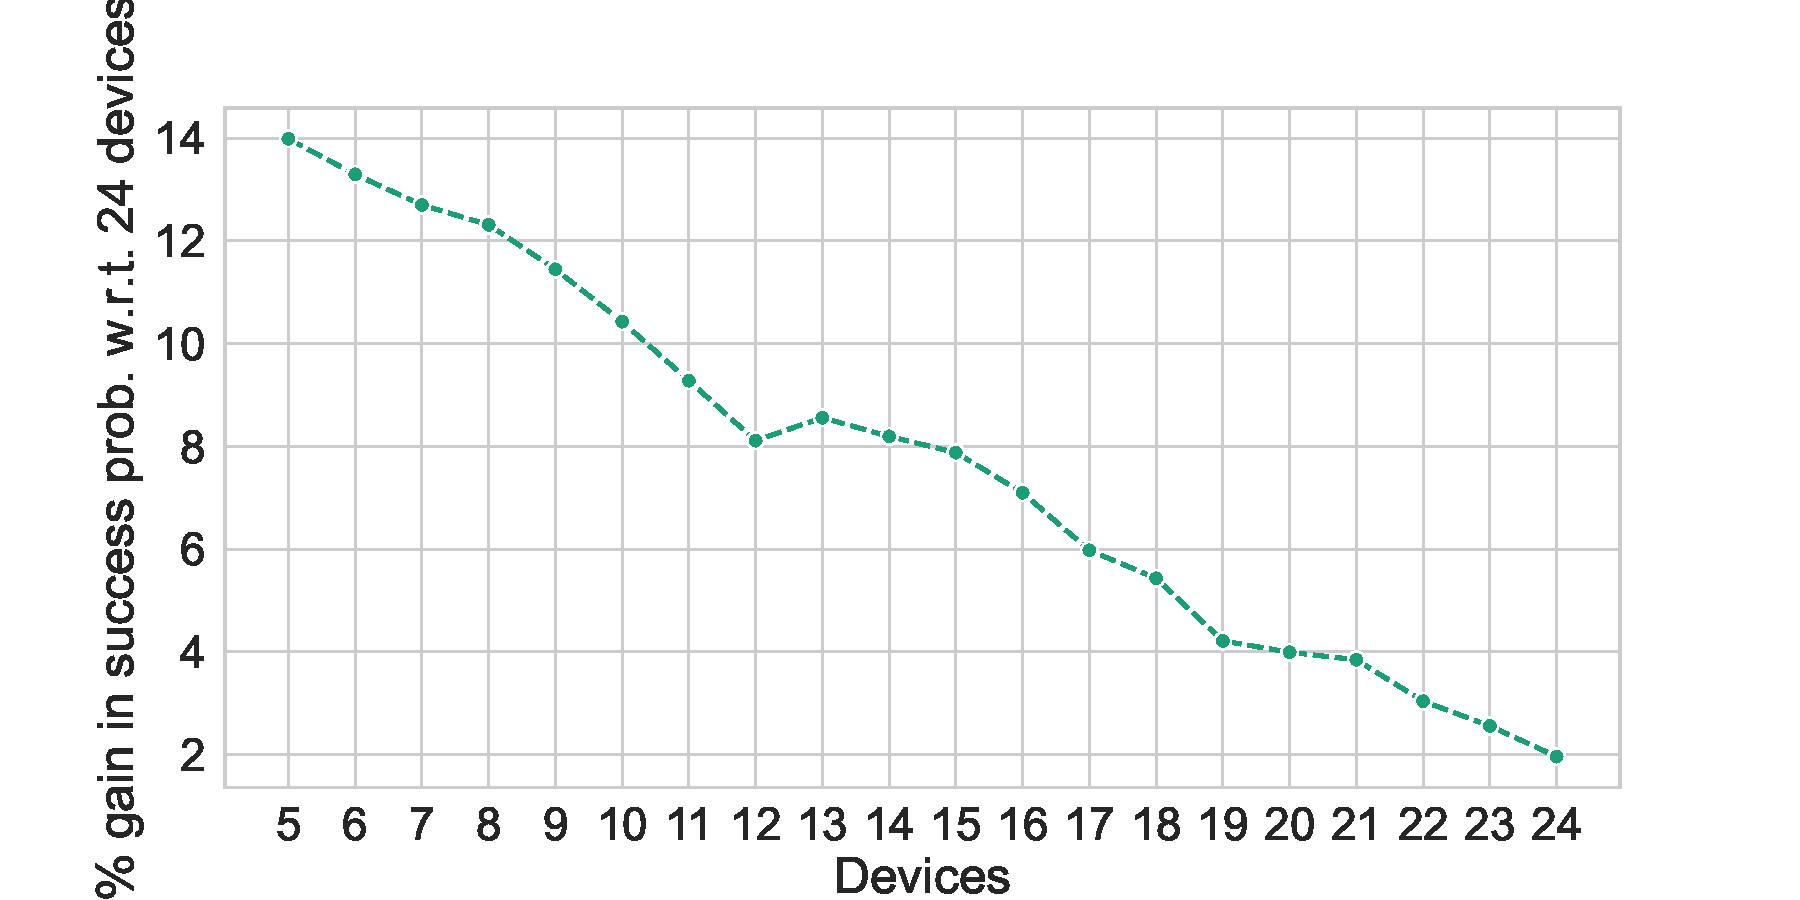
\includegraphics[scale = 0.4]{images/percentage_prob_wrt24_rolling4.pdf}
    \caption{Percentage gain in success probability w.r.t. 24 devices.}
    \label{fig:percentage_prob}
\end{figure*}
%But how can we measure its value? In order to do this, we have to define the so-called Value of Information. The value of an information product associated with a sensor service can be defined as its importance in the particular application usage context \cite{VoI}. After our analysis, we can suggest to take the accuracy obtained from different sensors of the logistic model as the starting point to develop a model for the Value Of Information. Further studies can be performed in order to build a model based on other metrics and to manage the trade-off between the accuracy and the amount of data that we are going to inject into the channel.
%As we have proved, selecting a smaller group of sensors allows us to be still able to perform binary classification at the receiver, but with a lower packet error rate, lower latencies and without overloading the network with a traffic that does not bring any addictional valuable information. As we have already seen, . Therefore, as a measure of the value of information, after our analysis, we can suggest to take the accuracy obtained for different sensors of the logistic model as the starting point to develop a model for the Value Of Information. Further studies can be performed in order to build a model based on other metrics and to manage the trade-off between the accuracy and the amount of data that we are going to inject into the channel.
\section{Further studies and possible improvements}

In addition to the simulation we performed, one could also consider to test NB-IoT technology. This possibility can be explored by means of the ongoing implementation of the new NB-IoT standard in ns-3 \cite{NB_IoT}. Nevertheless, we choose LoRaWAN since the NB-IoT is more suitable to static sensors, or in general, to sensors that are not constantly moving.

% and that generate bursty traffic, while we were looking for a technology that allowed us to transmit more often and almost in real-time. %Since it is still in development, we were not able to use it properly.

Another possible, yet simpler, approach is represented by adopting a modified version of the LENA \textit{lena-simple-epc.cc} example \cite{LENA} in NS-3, which can be adapted \cite{modify_LTE} to LTE-M technology for IoT. Such strategy is interesting as a first exploration of the problem, but it leads to trivial results in terms of throughput and mean delay.
%Comparisons with the different technologies can be performed in
Finally, further simulations could focus on making a performance comparison between LoRaWAN, NB-IoT technology and LTE-M technology.
%Moreover, since the applications have stric contraints about power consumption also this aspect could have been investigated.
\bibliography{bib}

\end{document}

